%-----------------------------------------------------------------------------
% Author: Rayla Kurosaki
% GitHub: https://github.com/rkp1503
%-----------------------------------------------------------------------------
\documentclass{rayla-project}
\usepackage{rayla-math-style}

%-----------------------------------------------------------------------------
% Project Information
%-----------------------------------------------------------------------------
\myUniversity{
    Rochester Institute of Technology\\
    College of Science\\
    School of Mathematical Sciences
    }
\myTitle{Bifurcation of Systems}
\myName{Ramsey (Rayla) Phuc}
\courseid{MATH-631.01}
\courseName{Dynamical Systems}
\professorName{Dr. Niels Otani}
\term{2021/08/23 - 2021/12/06}
\dueDate{2021/12/09}

%-----------------------------------------------------------------------------
% Start of Document
%-----------------------------------------------------------------------------
\begin{document}

    \maketitle

    %-------------------------------------------------------------------------
    % Abstract
    %-------------------------------------------------------------------------
    \begin{abstract}
        Bifurcation theory plays a fundamental role in understanding the qualitative behavior of dynamical systems. In this paper, we present a comprehensive study of various bifurcations within a carefully constructed system of equations. Our objective is to investigate the dynamic changes and transitions that occur as system parameters are varied. First, we establish a set of equations that capture the essential characteristics of the dynamical system under investigation. These equations are derived based on a thorough analysis of the underlying physical or mathematical phenomenon of interest. We ensure that the system exhibits nonlinear behavior and contains appropriate parameters to facilitate the exploration of bifurcations. Next, we employ analytical techniques to investigate the bifurcation points within the system. By analyzing the stability and eigenvalues of the system, we determine the types of bifurcations that arise, such as saddle-node, transcritical, pitchfork, and Hopf bifurcations. Furthermore, we utilize graphical tools, such as bifurcation diagrams and phase portraits, to visualize and interpret the bifurcation phenomena. In summary, this paper presents a systematic approach to construct a system of equations and investigates the bifurcations within it. Our findings contribute to the broader understanding of bifurcation theory and its applications, providing a valuable framework for exploring and analyzing the dynamic behavior of complex systems.
    \end{abstract}

    %-------------------------------------------------------------------------
    % Body
    %-------------------------------------------------------------------------
    \section{Introducing the system}\label{sec:introducing-the-system}
We will be constructing and analyzing a two-dimensional dynamical system that is in the form:
\begin{equation*}
    \begin{dcases}
        \begin{aligned}
            \diff[]{x}{t} &= f(x,y)\\
            \diff[]{y}{t} &= g(x,y)
        \end{aligned}
    \end{dcases}
\end{equation*}
under the conditions that this system should have:
\begin{enumerate}
    \item A minimum of two parameters
    \item A Hopf Bifurcation
    \item A Pitchfork Bifurcation (subcritical or supercritical)
    \item One other fixed point that is neither a Hopf Bifurcation nor a Pitchfork Bifurcation
    \item Either $f$ or $g$ must be a product of two or more functions
    \item Functional dependence that are substantial.
\end{enumerate}
The system that will be constructed and analyzed is:
\begin{equation}
    \begin{dcases}
        \begin{aligned}
            \diff[]{x}{t} &= f(x,y;\alpha,\beta,\gamma) = -\frac{1}{\alpha\beta}\left(\alpha+x^2-y\right)\left(\beta(x-1)+(x-1)^3-(y-1)\right)\left((1+\gamma)x-2y\right)\\
            \diff[]{y}{t} &= g(x,y) = x-y
        \end{aligned}
    \end{dcases}
    \label{eq:1}
\end{equation}

    \section{Constructing the system}\label{sec:constructing-the-system}

\subsection{Constructing a system that has a Saddle-Node Bifurcation}\label{subsec:constructing-a-system-that-has-a-saddle-node-bifurcation}
To start creating such a dynamical system, we will start by constructing a system that contains a Saddle-Node Bifurcation. Doing this will satisfy Condition 4. Consider the following system
\begin{equation*}
    \begin{dcases}
        \begin{aligned}
            \diff[]{x}{t} &= f_1(x,y;\alpha) = \alpha+x^2-y\\
            \diff[]{y}{t} &= g_1(x,y) = x-y
        \end{aligned}
    \end{dcases}
\end{equation*}
By inspection, Condition 6 is satisfied. Depending on the value of $\alpha$ in this system, we can have two, one, or zero fixed points given by:
\begin{equation*}
    \left(x^*,y^*\right) = \left\{\left(\frac{1-\sqrt{1-4\alpha}}{2}, \frac{1-\sqrt{1-4\alpha}}{2}\right), \left(\frac{1+\sqrt{1-4\alpha}}{2}, \frac{1+\sqrt{1-4\alpha}}{2}\right)\right\}
\end{equation*}
Note that if $\alpha<1/4$, then the term in the square root is positive. Thus, we have two distinct fixed points. At $\alpha=1/4$, the term in the square root vanishes, thus implying that there is only one fixed point. For $\alpha>1/4$, the term in the square root is negative. This implies that there are zero real fixed points. With this, we can conclude that this system has a Saddle-Node Bifurcation, satisfying Condition 4. \myref[Figure]{fig:1} provides a visual representation of the nullclines for different values of $\alpha$.

\subsection{Constructing a system that has a Pitchfork Bifurcation}\label{subsec:constructing-a-system-that-has-a-pitchfork-bifurcation}
Next we will move onto creating a system that contains a Pitchfork Bifurcation, thus satisfying Condition 3. Consider the following system
\begin{equation*}
    \begin{dcases}
        \begin{aligned}
            \diff[]{x}{t} &= f_2(x,y;\beta) = x^3-3x^2+(\beta+3)x-\beta-y\\
            \diff[]{y}{t} &= g_1(x,y) = x-y
        \end{aligned}
    \end{dcases}
\end{equation*}
By inspection, Condition 6 is satisfied. Depending on the value of $\beta$, we can have three, or one fixed points, which are given by:
\begin{equation*}
    \left(x^*,y^*\right) = \left\{\left(1, 1\right), \left(1-\sqrt{1-\beta}, 1-\sqrt{1-\beta}\right), \left(1+\sqrt{1-\beta}, 1+\sqrt{1-\beta}\right)\right\}
\end{equation*}
Note that if $\beta<1$, then the term in the square root will be positive implying that we have three distinct roots. If $\beta=1$, then the term in the square root will be zero implying that we have one distinct root. If $\beta>1$, then the term in the square root will be negative implying that we have 1 distinct root. This behavior tells us that we have a Subcritical Pitchfork Bifurcation, thus satisfying Condition 3. \myref[Figure]{fig:2} provides a visual representation of the nullclines for different values of $\beta$.

\subsection{Constructing a system that has a Hopf Bifurcation}\label{subsec:constructing-a-system-that-has-a-hopf-bifurcation}
Next, we will move onto creating a system that contains a Hopf Bifurcation in order to satisfy Condition 2. How do we do this? Consider the following arbitrary two-dimensional system:
\begin{equation*}
    \begin{dcases}
        \begin{aligned}
            \diff[]{x}{t} &= ax+by\\
            \diff[]{y}{t} &= cx+dy
        \end{aligned}
    \end{dcases}
\end{equation*}
Its Jacobian Matrix is:
\begin{equation*}
    \textbf{J} = \begin{bmatrix}
        a & b\\
        c & d
    \end{bmatrix}
\end{equation*}
Since we need a Hopf Bifurcation, we will want to have a center as a fixed point. Having a center as a fixed point implies that $\tau=0$ and $\Delta>0$. Thus, we need to satisfy $a=-d$ and $ad-bc>0$. If we choose $a=1$, then $d=-1$ and $bc<-1$. If we choose $c=1$, then $b<-1$. Lets choose $b=-2$. Then we have:
\begin{equation*}
    \begin{dcases}
        \begin{aligned}
            \diff[]{x}{t} &= f(x,y) = x-2y\\
            \diff[]{y}{t} &= g(x,y) = x-y
        \end{aligned}
    \end{dcases}
\end{equation*}
From here, we will add another parameter that will change the value of $\tau$. Consider the following system:
\begin{equation*}
    \begin{dcases}
        \begin{aligned}
            \diff[]{x}{t} &= f_3(x,y;\gamma) = (1+\gamma)x-2y\\
            \diff[]{y}{t} &= g_1(x,y) = x-y
        \end{aligned}
    \end{dcases}
\end{equation*}
For this particular system, we will have different values of $\gamma$ that can change the type of fixed point. If $\gamma<0$, then we have a stable spiral. If $\gamma=0$, then we have a center. If $\gamma>0$ but $\gamma<1$, then we have an unstable spiral. If $\gamma=1$, then we have a line of fixed points. Finally, for $\gamma>1$, we have a saddle point. \myref[Figure]{fig:3} provides a visual representation of the system for different values of $\gamma$.

\subsection{Finalizing the system}\label{subsec:finalizing-the-system}
Now we have three different systems where each one has a particular Bifurcation. To create a system that contains all three of these bifurcations, we will multiply the respective $f$ functions together and the respective $g$ functions together. This gives us:
\begin{equation*}
    \begin{dcases}
    \begin{aligned}
        \diff[]{x}{t} &= f(x,y;\alpha,\beta,\gamma) = \left(\alpha+x^2-y\right)\left(\beta(x-1)+(x-1)^3-(y-1)\right)\left((1+\gamma)x-2y\right)\\
        \diff[]{y}{t} &= g(x,y) = x-y
    \end{aligned}
    \end{dcases}
\end{equation*}
By inspection, Conditions 1, 5, and 6 are satisfied. Since Condition 5 is satisfied, Conditions 2, 3, and 4 are also satisfied based on the previous analysis. To finalize the system, we will divide both $f$ and $g$ by $f_1(0,0)f_2(0,0)$ to prevent any potential problems when computing the Jacobian Matrix of this system. Here, $f_1f_2$ at $(0,0)$ is $-\alpha\beta$, which changes our system to:
\begin{equation*}
    \begin{dcases}
    \begin{aligned}
        \diff[]{x}{t} &= f(x,y;\alpha,\beta,\gamma) = -\frac{1}{\alpha\beta}\left(\alpha+x^2-y\right)\left(\beta(x-1)+(x-1)^3-(y-1)\right)\left((1+\gamma)x-2y\right)\\
        \diff[]{y}{t} &= g(x,y) = x-y
    \end{aligned}
    \end{dcases}
\end{equation*}
Thus, \myref[System]{eq:1} is a valid two-dimensional system we can analyze that satisfies the six conditions listed above.

    \section{Computing the Jacobian Matrix of the system}\label{sec:computing-the-jacobian-matrix-of-the-system}
The expanded form of $f(x,y;\alpha,\beta,\gamma)$ is:
\begin{align*}
    f(x,y;\alpha,\beta,\gamma) &= (\gamma+1)x^6 - 2x^5y - 3(\gamma+1)x^5 + \left(5-\gamma\right)x^4y + \left(\alpha+\beta+3\right)(\gamma+1)x^4 + 2x^3y^2\\
    &+ 2\left(\gamma-\alpha-\beta-2\right)x^3y - \left(3\alpha+\beta\right)(\gamma+1)x^3 - 4x^2y^2 + \left(6\alpha-(\beta+3)(\gamma+1)\right)x^2y\\
    &+ \alpha\left(3+\beta\right)(\gamma+1)x^2 + \left(2\beta+\gamma+7\right)xy^2 - \left(2\alpha(\beta+\gamma)+7\alpha-\beta(\gamma+1)\right)xy - \alpha\beta(\gamma+1)x\\
    &- 2y^3 + 2\left(\alpha-\beta\right)y^2 + 2\alpha\beta y
\end{align*}
Its partial derivatives with respect to $x$ and $y$ are:
\begin{align*}
    \pdiff[]{f}{x} &= 6(\gamma+1)x^5 - 10x^4y - 15(\gamma+1)x^4 + 4\left(5-\gamma\right)x^3y + 4\left(\alpha+\beta+3\right)(\gamma+1)x^3 + 6x^2y^2\\
    &+ 6\left(\gamma-\alpha-\beta-2\right)x^2y - 3\left(3\alpha+\beta\right)(\gamma+1)x^2 - 8xy^2 + 2\left(6\alpha-(\beta+3)(\gamma+1)\right)xy + 2\alpha\left(3+\beta\right)(\gamma+1)x\\
    &+ \left(2\beta+\gamma+7\right)y^2 - \left(2\alpha(\beta+\gamma)+7\alpha-\beta(\gamma+1)\right)y - \alpha\beta(\gamma+1)\\
    \pdiff[]{f}{y} &= - 2x^5 + \left(5-\gamma\right)x^4 + 4x^3y + 2\left(\gamma-\alpha-\beta-2\right)x^3 - 8x^2y + \left(6\alpha-(\beta+3)(\gamma+1)\right)x^2 + 2\left(2\beta+\gamma+7\right)xy\\
    &- \left(2\alpha(\beta+\gamma)+7\alpha-\beta(\gamma+1)\right)x - 6y^2 + 4\left(\alpha-\beta\right)y + 2\alpha\beta
\end{align*}
So the Jacobian Matrix for this system is:
\begin{equation}
    \textbf{J} = \begin{bmatrix}
        \pdiff[]{f}{x} & \pdiff[]{f}{y}\\
        1 & -1
    \end{bmatrix}
    \label{eq:2}
\end{equation}

    \section{Analyzing the system for a default set of parameters}\label{sec:analyzing-the-system-for-a-default-set-of-parameters}
Let's consider the system when $\alpha=-1,\beta=1,\gamma=0$:
\begin{equation}
    \begin{dcases}
        \begin{aligned}
            \diff[]{x}{t} &= f(x,y;-1,1,0) = \left(x^2-1-y\right)\left((x-1)+(x-1)^3-(y-1)\right)\left(x-2y\right)\\
            \diff[]{y}{t} &= g(x,y;-1,1) = x-y
        \end{aligned}
    \end{dcases}
    \label{eq:4}
\end{equation}

\subsection{Equations to solve to find all fixed points}\label{subsec:equations-to-solve-to-find-all-fixed-points}
In order to find all the fixed points, we will need to solve the following equations:
\begin{equation*}
    \begin{dcases}
        \begin{aligned}
            x &= x^2-1\\
            x &= (x-1)+(x-1)^3+1\\
            x &= \frac{x}{2}
        \end{aligned}
    \end{dcases}
\end{equation*}

\subsection{Analyzing all fixed points via the Jacobian Matrix}\label{subsec:analyzing-all-fixed-points-via-the-jacobian-matrix}
Using the provided software and the prior analysis, the fixed points for this system are:
\begin{equation*}
    \left(x^*,y^*\right) = \left\{\left(\frac{1-\sqrt{5}}{2}, \frac{1-\sqrt{5}}{2}\right), \left(0,0\right), \left(1,1\right), \left(\frac{1+\sqrt{5}}{2}, \frac{1+\sqrt{5}}{2}\right)\right\}
\end{equation*}
For this system, the Jacobian matrix is:
\begin{equation*}
    \textbf{J} = \begin{bmatrix}
        \pdiff[]{f}{x} & \pdiff[]{f}{y}\\
        1 & -1
    \end{bmatrix}
\end{equation*}
where
\begin{align*}
    \pdiff[]{f}{x} &= 6x^5-10x^4y-15x^4+20x^3y+12x^3+6x^2y^2-12x^2y+6x^2-8xy^2-16xy-8x+9y^2+10y+1\\
    \pdiff[]{f}{y} &= -2x^5+5x^4+4x^3y-4x^3-8x^2y-8x^2+18xy+10x-6y^2-8y-2
\end{align*}
Lets give these fixed points names:
\begin{equation*}
    P_1=\left(\frac{1-\sqrt{5}}{2}, \frac{1-\sqrt{5}}{2}\right),\quad P_2=\left(0,0\right),\quad P_3=\left(1,1\right),\quad P_4=\left(\frac{1+\sqrt{5}}{2}, \frac{1+\sqrt{5}}{2}\right)
\end{equation*}
For the four fixed points, the Jacobian Matrix, their traces and determinants are:
\begin{alignat*}{3}
    P_1:&\quad \textbf{J} = \begin{bmatrix}
        1+\sqrt{5} & \frac{3+\sqrt{5}}{2}\\
        1 & -1
    \end{bmatrix} &&\implies \begin{dcases}
    \begin{aligned}
        \tau &= \sqrt{5}>0\\
        \Delta &= -\frac{5+3\sqrt{5}}{2}<0
    \end{aligned}
    \end{dcases}\\
    P_2:&\quad \textbf{J} = \begin{bmatrix}
        1 & -2\\
        1 & -1
    \end{bmatrix} &&\implies \begin{dcases}
    \begin{aligned}
        \tau &= 0\\
        \Delta &= 1>0
    \end{aligned}
    \end{dcases}\\
    P_3:&\quad \textbf{J} = \begin{bmatrix}
        1 & -1\\
        1 & -1
    \end{bmatrix} &&\implies \begin{dcases}
    \begin{aligned}
        \tau &= 0\\
        \Delta &= 0
    \end{aligned}
    \end{dcases}\\
    P_4:&\quad \textbf{J} = \begin{bmatrix}
        1-\sqrt{5} & \frac{3-\sqrt{5}}{2}\\
        1 & -1
    \end{bmatrix} &&\implies \begin{dcases}
    \begin{aligned}
        \tau &= -\sqrt{5}<0\\
        \Delta &= \frac{-5+3\sqrt{5}}{2}>0
    \end{aligned}
    \end{dcases}
\end{alignat*}
Here we can classify some of these fixed points. For $P_1$, since $\Delta<0$, this implies that $P_1$ is a Saddle Node. Also, since $\tau>0$, this implies that $P_1$ is Unstable. Therefore $P_1$ is an Unstable Saddle Node. For $P_2$, since $\Delta>0$ and $\tau^2-4\Delta<0$, this implies that we have a Center. Furthermore, since $\tau=0$, this implies that $P_2$ is Neutrally Stable. Therefore, $P_2$ is a Neutrally Stable Center. For $P_3$, we have $\tau=\Delta=0$. Since this system is a nonlinear system, we cannot draw any conclusions about the type of fixed point $P_3$ is based on this analysis alone. We will need to do more work. Using the software provided, we will look into trajectories close to $P_3$. Based on \figref{fig:4}, we can say that $P_3$ is a Saddle-Node. For $P_4$, since $\Delta>0$ and $\tau^2-4\Delta>0$, this implies that $P_4$ is a Node. Furthermore, since $\tau<0$, this implies that $P_4$ is Stable. Therefore, $P_4$ is a Stable Node.

\subsection{Computing Eigenvalues and Eigenvectors for all fixed points}\label{subsec:computing-eigenvalues-and-eigenvectors-for-all-fixed-points}
Now we will find the eigenvalues and their corresponding eigenvectors for all fixed points present in the system. Starting with $P_1$ the eigenvalues are:
\begin{align*}
    p(\lambda) &= \det\left(\textbf{J}-\lambda I\right) = \begin{vmatrix}
        1+\sqrt{5}-\lambda & \frac{3+\sqrt{5}}{2}\\
        1 & -1-\lambda
    \end{vmatrix}\\
    0 &= (1+\sqrt{5}-\lambda)(-1-\lambda)-1\left(\frac{3+\sqrt{5}}{2}\right)\\
    0 &= \lambda^2-\sqrt{5}\lambda - \frac{5+3\sqrt{5}}{2}\\
    \implies \lambda &= \frac{-\left(-\sqrt{5}\right) \pm \sqrt{\left(-\sqrt{5}\right)^2-4(1)\left(-\frac{5+3\sqrt{5}}{2}\right)}}{2(1)}\\
    \Aboxed{\lambda &= \left\{\frac{\sqrt{5} - \sqrt{15+6\sqrt{5}}}{2}, \frac{\sqrt{5} + \sqrt{15+6\sqrt{5}}}{2}\right\} = \{-1.5473, 3.7834\}}
\end{align*}
and their respective eigenvectors are:
\begin{align*}
    \vec{v} &= \left\{\begin{bmatrix}
        \frac{3+\sqrt{5}}{2}\\
        -\left(1+\sqrt{5}-\frac{\sqrt{5} - \sqrt{15+6\sqrt{5}}}{2}\right)
    \end{bmatrix}, \begin{bmatrix}
        \frac{3+\sqrt{5}}{2}\\
        -\left(1+\sqrt{5}-\frac{\sqrt{5} + \sqrt{15+6\sqrt{5}}}{2}\right)
    \end{bmatrix}\right\}\\
    \Aboxed{\vec{v} &= \left\{\begin{bmatrix}
        \frac{3+\sqrt{5}}{2}\\
        \frac{\sqrt{5} - \sqrt{15+6\sqrt{5}}}{2}-1-\sqrt{5}
    \end{bmatrix}, \begin{bmatrix}
        \frac{3+\sqrt{5}}{2}\\
        \frac{\sqrt{5} + \sqrt{15+6\sqrt{5}}}{2}-1-\sqrt{5}
    \end{bmatrix}\right\} = \left\{\begin{bmatrix}
        2.6180\\
        -4.7834
    \end{bmatrix}, \begin{bmatrix}
        2.6180\\
        0.5473
    \end{bmatrix}\right\}}
\end{align*}
For $P_2$, the eigenvalues are:
\begin{align*}
    p(\lambda) &= \det\left(\textbf{J}-\lambda I\right) = \begin{vmatrix}
        1-\lambda & -2\\
        1 & -1-\lambda
    \end{vmatrix}\\
    0 &= (1-\lambda)(-1-\lambda)-1(-2)\\
    0 &= \lambda^2+1\\
    \implies \Aboxed{\lambda &= \left\{-i, i\right\}}
\end{align*}
and their respective eigenvectors are:
\begin{align*}
    \vec{v} &= \left\{\begin{bmatrix}
        -2\\
        -\left(1+i\right)
    \end{bmatrix}, \begin{bmatrix}
        -2\\
        -\left(1-i\right)
    \end{bmatrix}\right\}\\
    \Aboxed{\vec{v} &= \left\{\begin{bmatrix}
        -2\\
        -1-i
    \end{bmatrix}, \begin{bmatrix}
        -2\\
        i-1
    \end{bmatrix}\right\}}
\end{align*}
Since we have complex eigenvalue and complex eigenvectors, this implies that the fixed point is either a spiral or a center, which has a sense of rotation. The flow for this fixed point rotates clockwise.\\
For $P_3$, the eigenvalues are:
\begin{align*}
    p(\lambda) &= \det\left(\textbf{J}-\lambda I\right) = \begin{vmatrix}
        1-\lambda & -1\\
        1 & -1-\lambda
    \end{vmatrix}\\
    0 &= (1-\lambda)(-1-\lambda)-1(-1)\\
    0 &= \lambda^2\\
    \implies \Aboxed{\lambda &= \left\{0\right\}}
\end{align*}
and their respective eigenvectors are:
\begin{align*}
    \vec{v} &= \left\{\begin{bmatrix}
        -1\\
        -\left(1\right)
    \end{bmatrix}\right\}\\
    \Aboxed{\vec{v} &= \left\{\begin{bmatrix}
        -1\\
        -1
    \end{bmatrix}\right\}}
\end{align*}
For $P_4$, the eigenvalues are:
\begin{align*}
    p(\lambda) &= \det\left(\textbf{J}-\lambda I\right) = \begin{vmatrix}
        1-\sqrt{5}-\lambda & \frac{3-\sqrt{5}}{2}\\
        1 & -1-\lambda
    \end{vmatrix}\\
    0 &= (1-\sqrt{5}-\lambda)(-1-\lambda)-1\left(\frac{3-\sqrt{5}}{2}\right)\\
    0 &= \lambda^2+\sqrt{5}\lambda+\frac{-5+3\sqrt{5}}{2}\\
    \implies \lambda &= \frac{-\left(\sqrt{5}\right) \pm \sqrt{\left(\sqrt{5}\right)^2-4\left(\sqrt{5}\right)\left(\frac{-5+3\sqrt{5}}{2}\right)}}{2\left(1\right)}\\
    \Aboxed{\lambda &= \left\{\frac{-\sqrt{5}-\sqrt{15-6\sqrt{5}}}{2}, \frac{-\sqrt{5}+\sqrt{15-6\sqrt{5}}}{2}\right\} = \left\{-1.7472, -0.4888\right\}}
\end{align*}
and their respective eigenvectors are:
\begin{align*}
    \vec{v} &= \left\{\begin{bmatrix}
        \frac{3-\sqrt{5}}{2}\\
        -\left(1-\sqrt{5}-\frac{-\sqrt{5}-\sqrt{15-6\sqrt{5}}}{2}\right)
    \end{bmatrix}, \begin{bmatrix}
        \frac{3-\sqrt{5}}{2}\\
        -\left(1-\sqrt{5}-\frac{-\sqrt{5}+\sqrt{15-6\sqrt{5}}}{2}\right)
    \end{bmatrix}\right\}\\
    \Aboxed{\vec{v} &= \left\{\begin{bmatrix}
        \frac{3-\sqrt{5}}{2}\\
        \sqrt{5}-1-\frac{\sqrt{5}+\sqrt{15-6\sqrt{5}}}{2}
    \end{bmatrix}, \begin{bmatrix}
        \frac{3-\sqrt{5}}{2}\\
        \sqrt{5}-1+\frac{-\sqrt{5}+\sqrt{15-6\sqrt{5}}}{2}
    \end{bmatrix}\right\} = \left\{\begin{bmatrix}
        0.3820\\
        -0.5112
    \end{bmatrix}, \begin{bmatrix}
        0.3820\\
        0.7472
    \end{bmatrix}\right\}}
\end{align*}

\subsection{Graphical representation of the system}\label{subsec:graphical-representation-of-the-system}
\figref{fig:5} shows the nullclines for the system with these sets of parameters. \figref{fig:6} shows the phase portrait for the system with these sets of parameters. It contains all the fixed points, trajectories to show the overall flow, arrows to indicate the direction of the flow with increasing time, eigenvector directions, and manifolds.

\subsection{Graphical analysis of the system}\label{subsec:graphical-analysis-of-the-system}
We have one fixed point that has complex eigenvalues, which is $(0,0)$. Referring to \figref{fig:8}, we can see that sense of rotation near this fixed point is clockwise, which is what we predicted in Section 4.3. We have one fixed point that is a Stable Node, which is the fixed point $\left(\frac{1+\sqrt{5}}{2}, \frac{1+\sqrt{5}}{2}\right)$. For this Stable Node, there are trajectories that go along one of the eigenvector directions.

    \section{Hopf Bifurcation analysis}\label{sec:hopf-bifurcation-analysis}

\subsection{Subcritical or Supercritical?}\label{subsec:subcritical-or-supercritical?}
We know that the system contains a Hopf Bifurcation. We will determine whether it is a Subcritical Hopf Bifurcation or a Supercritical Hopf Bifurcation by generating two phase portraits and comparing them. \figref{fig:9} is a phase portrait of the system before the bifurcation and \figref{fig:10} is a phase portrait of the system just after the bifurcation. For both figures, we will zoom in closer to the fixed point $(0,0)$ and plot a trajectory that goes through the point $(-0.1,-0.1)$. From these figures, we can conclude that the Hopf Bifurcation is a Subcritical Hopf Bifurcation.

\subsection{Parameter analysis}\label{subsec:parameter-analysis}
Here, we can guess that the Hopf Bifurcation occurs at $\gamma=0$. To verify this, we will take the Jacobian of the System for an arbitrary $\gamma$, evaluated at $(0,0)$:
\begin{align*}
    \textbf{J} &= \begin{bmatrix}
        1+\gamma & -2\\
        1 & -1
    \end{bmatrix}
\end{align*}
From here, we can determine that the trace of the system is $\tau=\gamma$ which implies that the behavior of the system near $(0,0)$ changes when $\gamma<0$ and when $\gamma>0$. Thus, $\gamma=0$ is where the Hopf Bifurcation occurs.

    \section{Pitchfork Bifurcation analysis}\label{sec:pitchfork-bifurcation-analysis}

\subsection{Plots}\label{subsec:plots}
To analyze the Pitchfork Bifurcation in this system, we will fix $\alpha$ and $\gamma$ and we will choose values for $\beta$ where $\beta\neq0$. Here, we will choose the case where $\beta=\pm2$.


    %-------------------------------------------------------------------------
    % Bibliography
    %-------------------------------------------------------------------------
    \newpage
    % \nocite{*}
    \printbibliography[title={Bibliography}]

    %-------------------------------------------------------------------------
    % Appendix
    %-------------------------------------------------------------------------
    \newpage
    \appendix
    \section{Figures}\label{sec:figures}

\begin{figure}[H]
    \centering
    \begin{subfigure}{.32\textwidth}
        \centering
        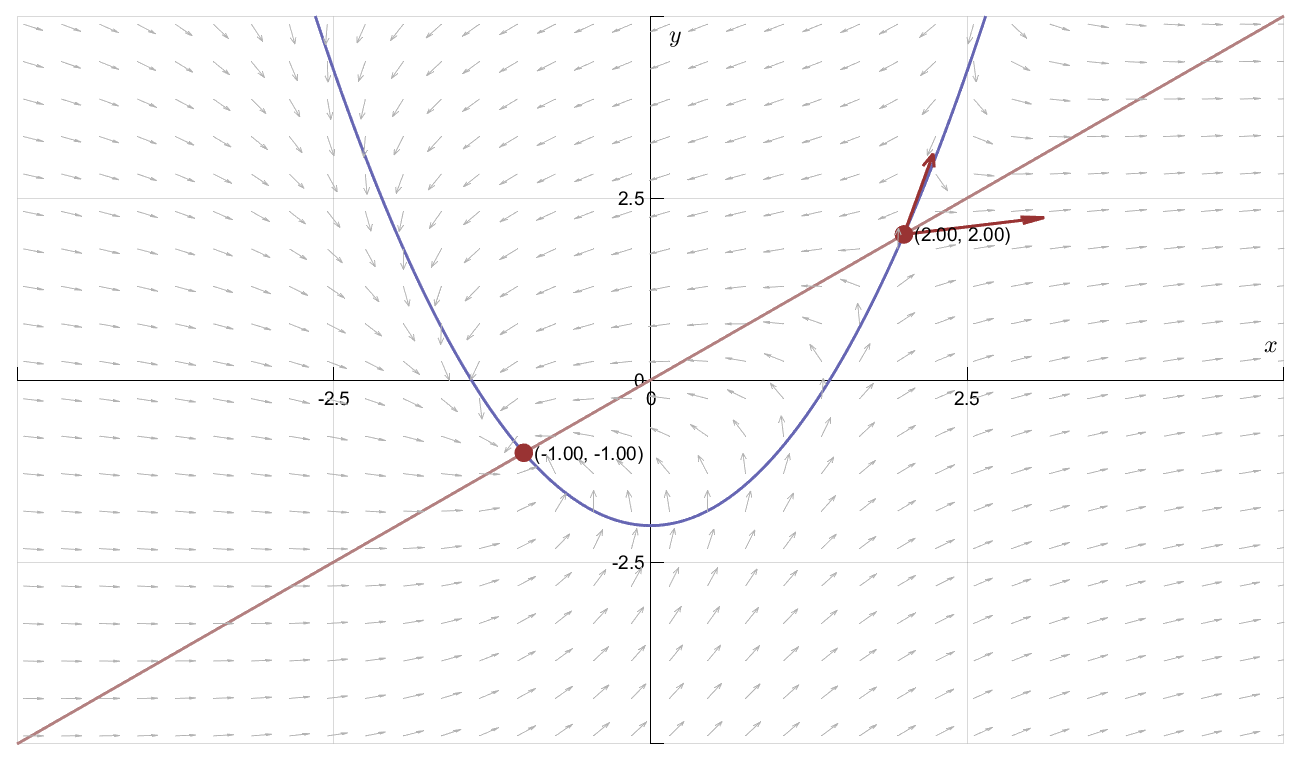
\includegraphics[width=\textwidth]{fig2.1_a.png}
        \caption{$\alpha=-2$}
    \end{subfigure}
    \begin{subfigure}{.32\textwidth}
        \centering
        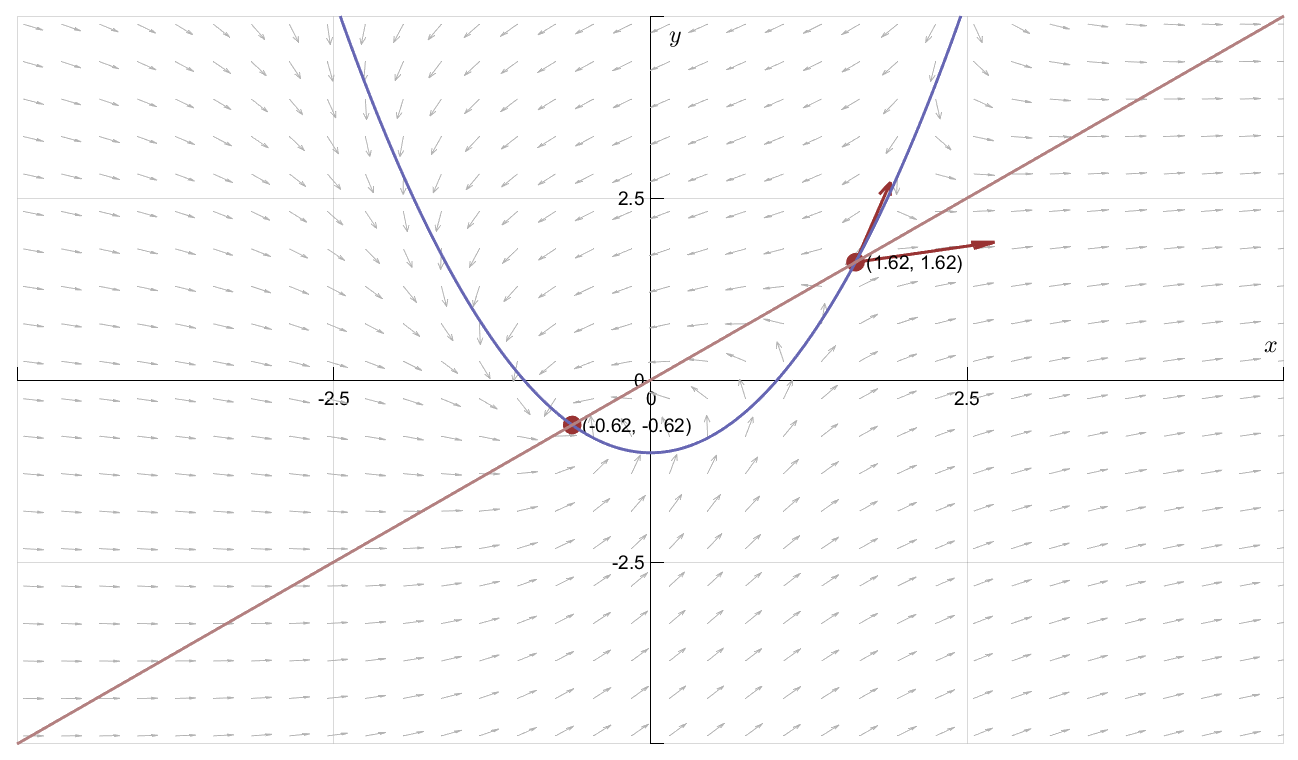
\includegraphics[width=\textwidth]{fig2.1_b.png}
        \caption{$\alpha=-1$}
    \end{subfigure}
    \begin{subfigure}{.32\textwidth}
        \centering
        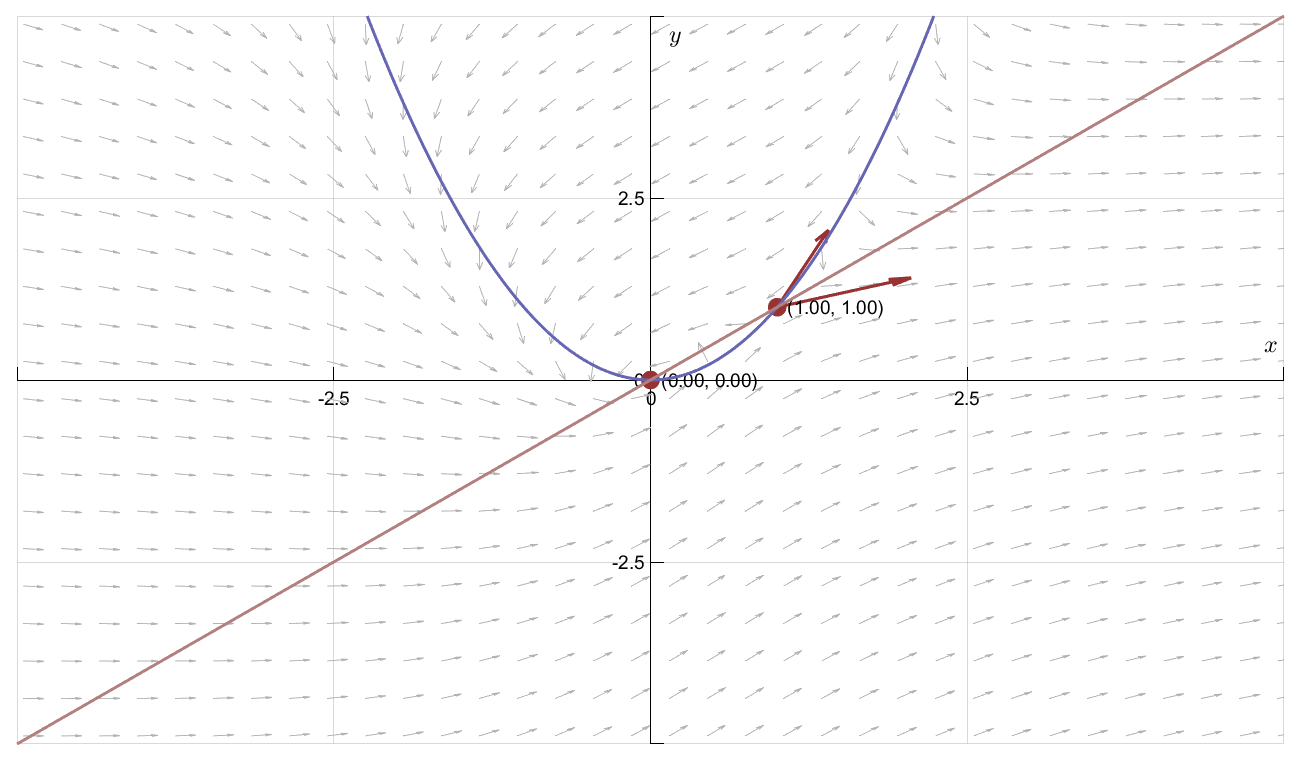
\includegraphics[width=\textwidth]{fig2.1_c.png}
        \caption{$\alpha=0$}
    \end{subfigure}
    \begin{subfigure}{.49\textwidth}
        \centering
        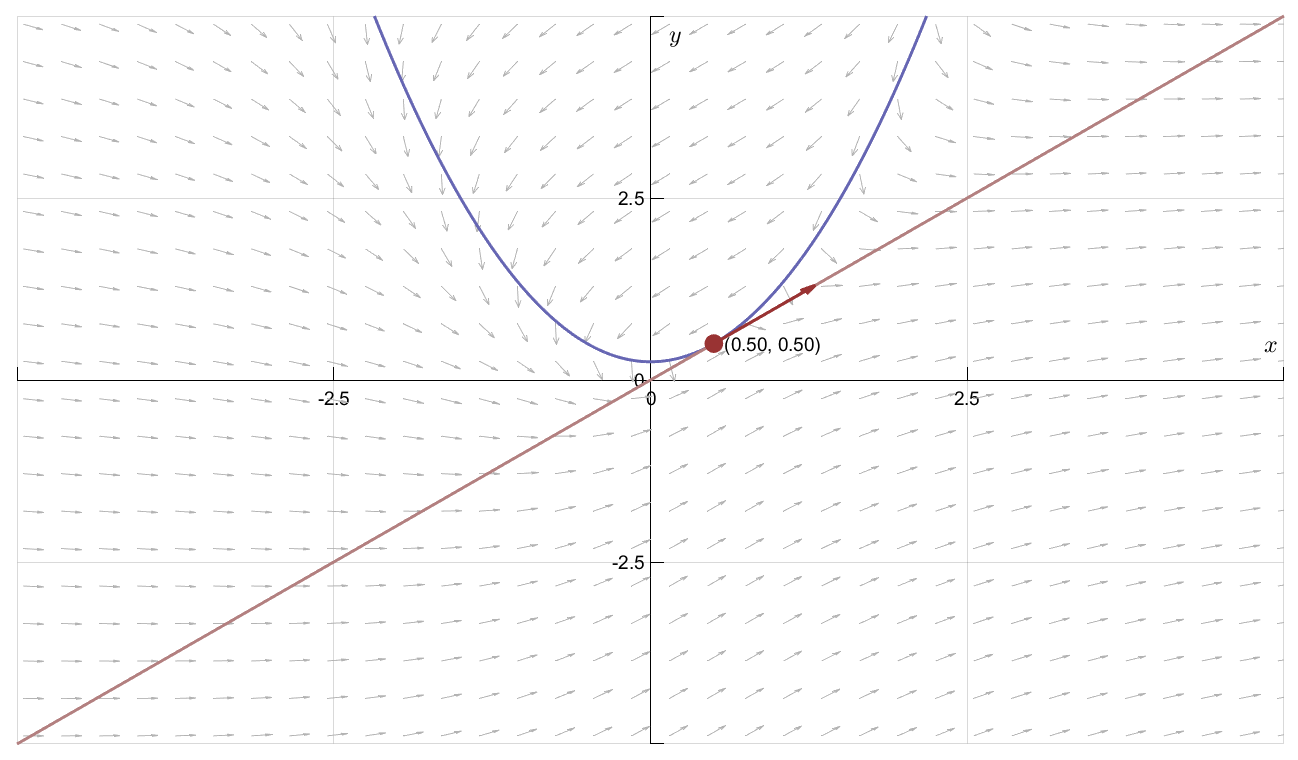
\includegraphics[width=\textwidth]{fig2.1_d.png}
        \caption{$\alpha=1/4$}
    \end{subfigure}
    \begin{subfigure}{.49\textwidth}
        \centering
        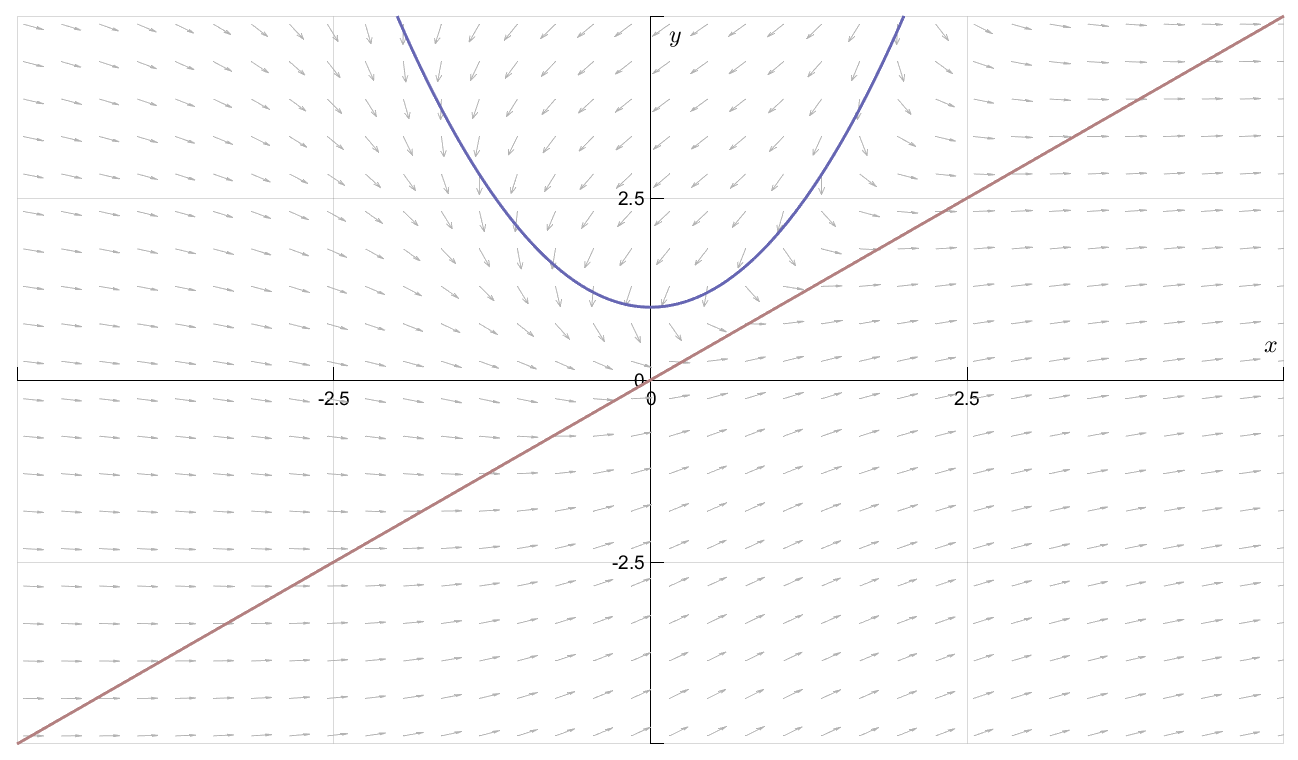
\includegraphics[width=\textwidth]{fig2.1_e.png}
        \caption{$\alpha=1$}
    \end{subfigure}
    \caption{Nullcline Analysis for potential system 1}
    \label{fig:1}
\end{figure}

\begin{figure}[H]
    \centering
    \begin{subfigure}{.32\textwidth}
        \centering
        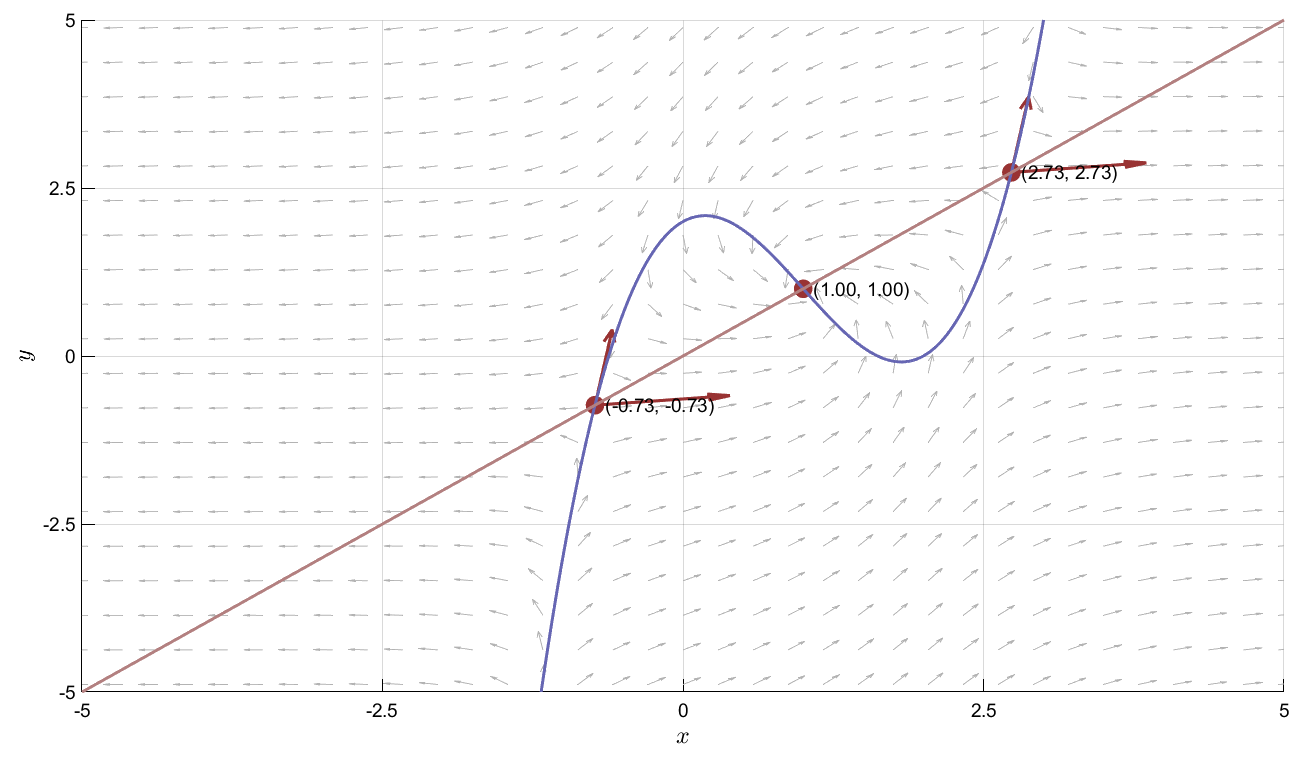
\includegraphics[width=\textwidth]{fig2.2_a.png}
        \caption{$\beta=-2$}
    \end{subfigure}
    \begin{subfigure}{.32\textwidth}
        \centering
        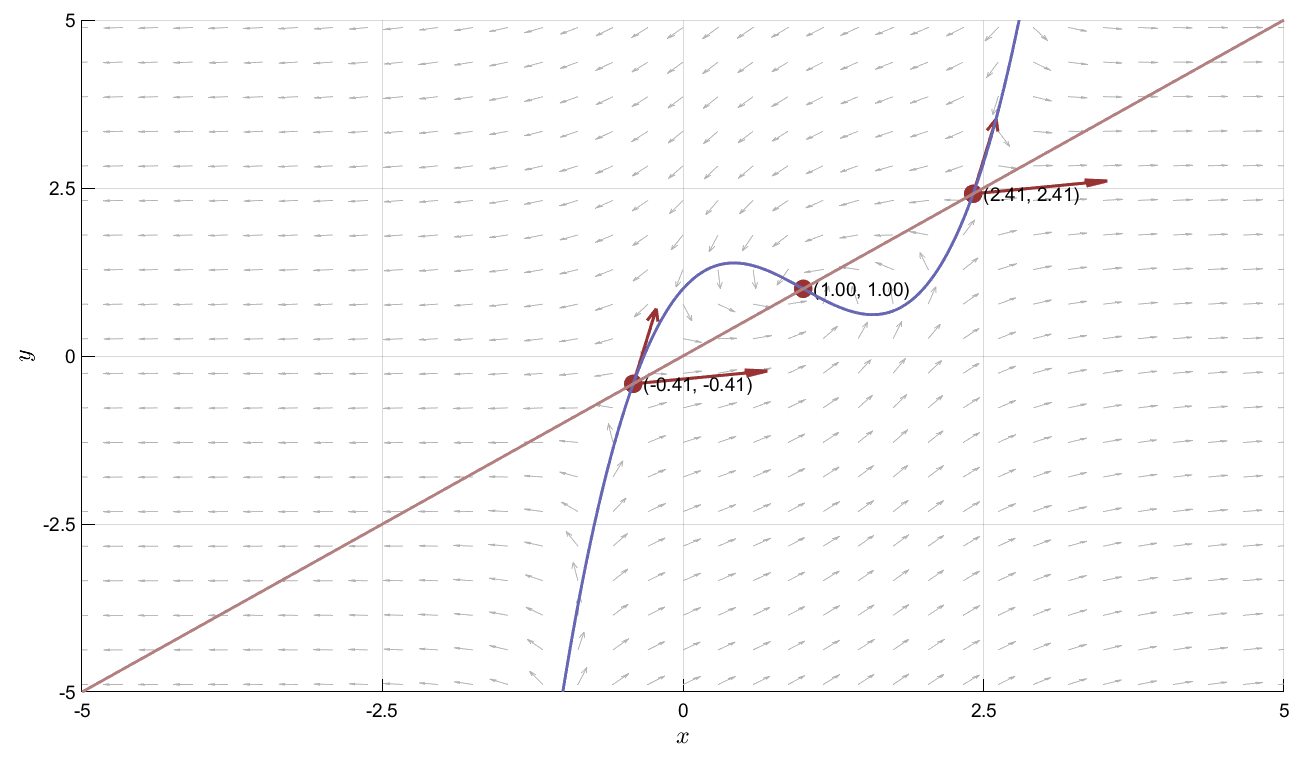
\includegraphics[width=\textwidth]{fig2.2_b.png}
        \caption{$\beta=-1$}
    \end{subfigure}
    \begin{subfigure}{.32\textwidth}
        \centering
        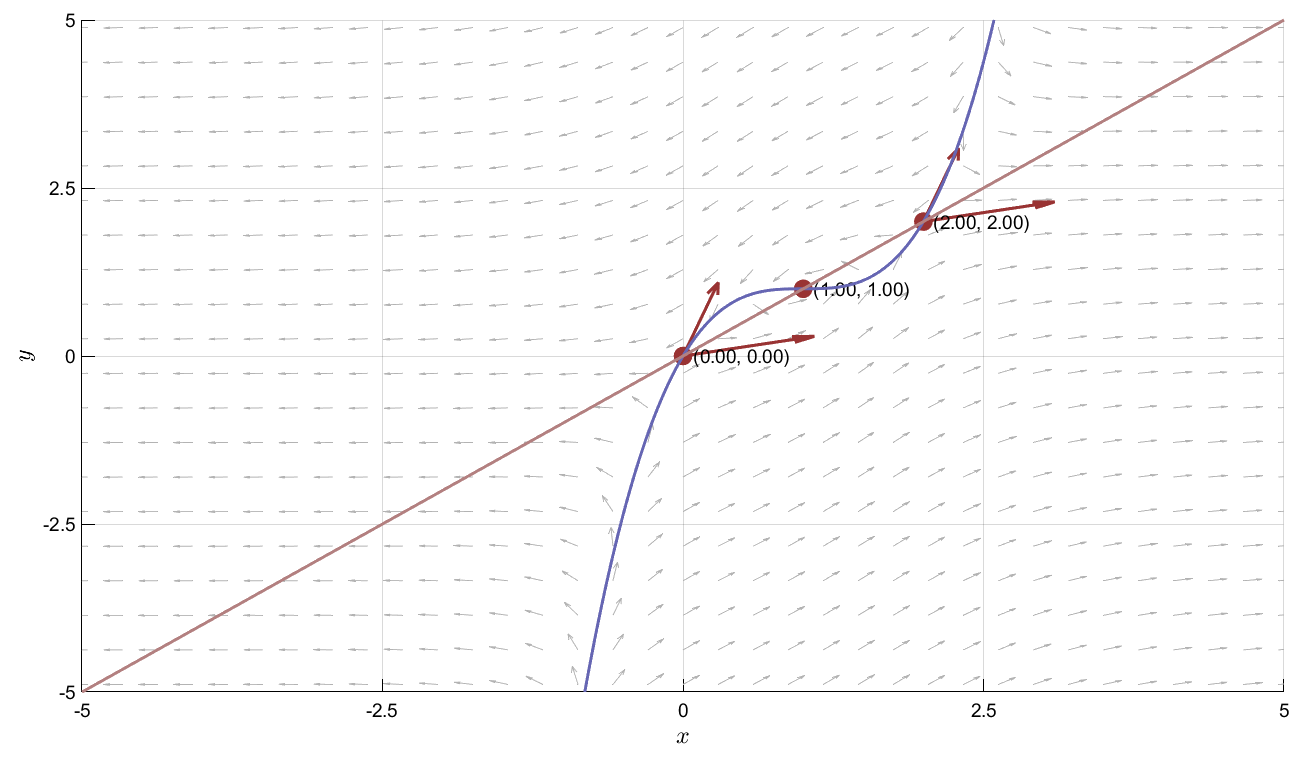
\includegraphics[width=\textwidth]{fig2.2_c.png}
        \caption{$\beta=0$}
    \end{subfigure}
    \begin{subfigure}{.49\textwidth}
        \centering
        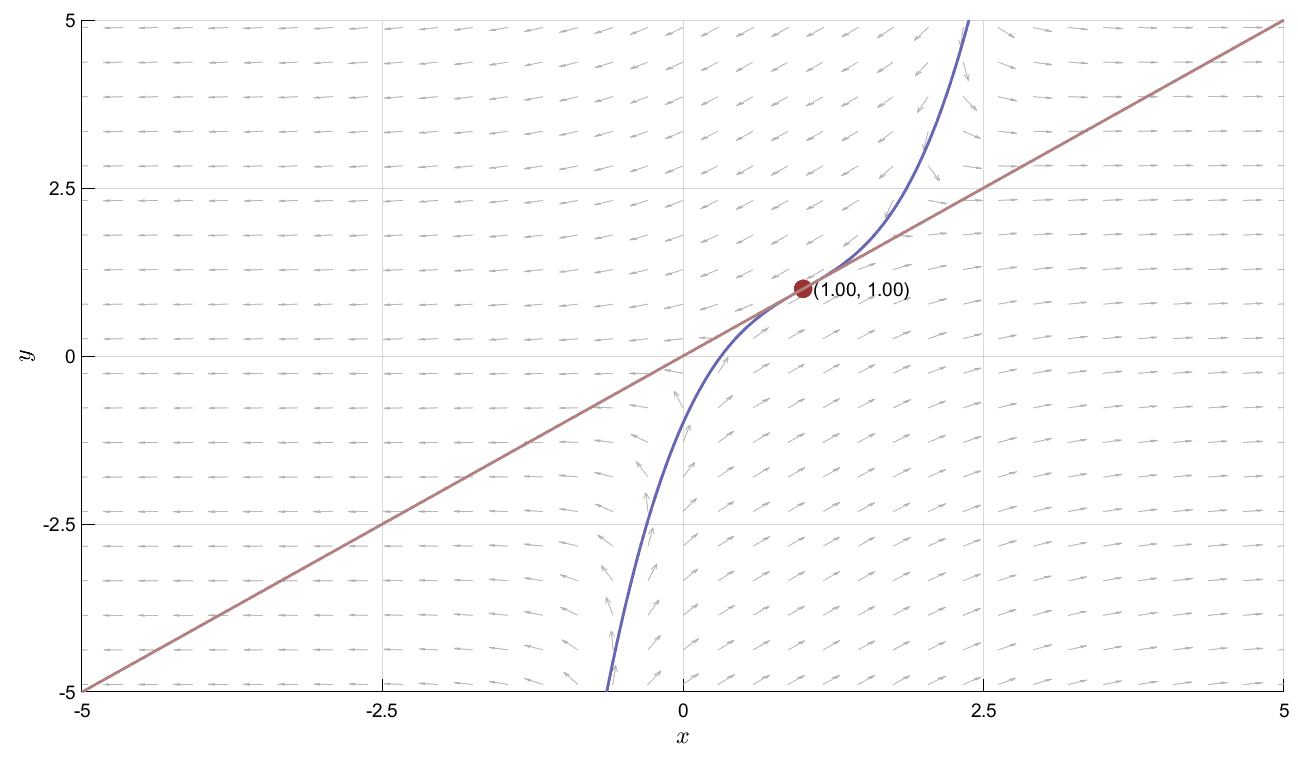
\includegraphics[width=\textwidth]{fig2.2_d.png}
        \caption{$\beta=1$}
    \end{subfigure}
    \begin{subfigure}{.49\textwidth}
        \centering
        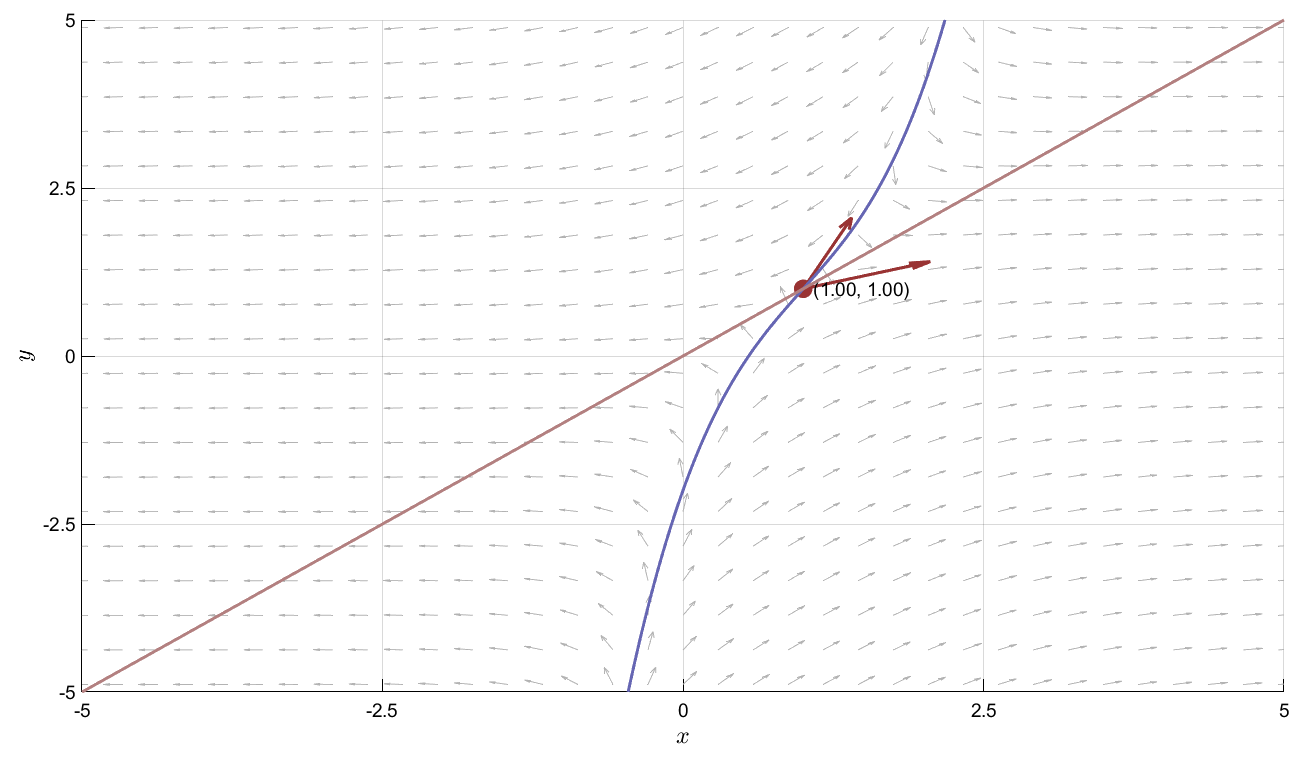
\includegraphics[width=\textwidth]{fig2.2_e.png}
        \caption{$\beta=2$}
    \end{subfigure}
    \caption{Nullcline Analysis for potential system 2}
    \label{fig:2}
\end{figure}

\begin{figure}[H]
    \centering
    \begin{subfigure}{.32\textwidth}
        \centering
        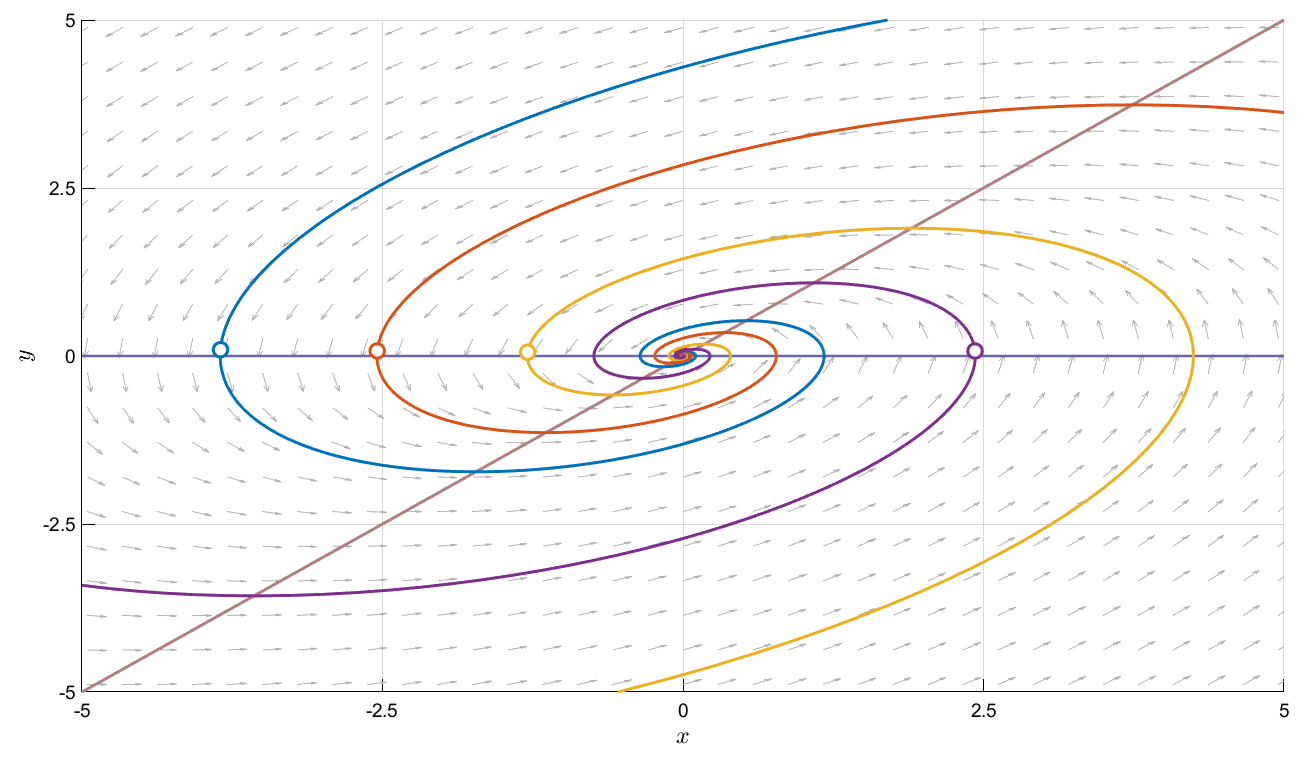
\includegraphics[width=\textwidth]{fig2.3_a.png}
        \caption{$\gamma=-1$}
    \end{subfigure}
    \begin{subfigure}{.32\textwidth}
        \centering
        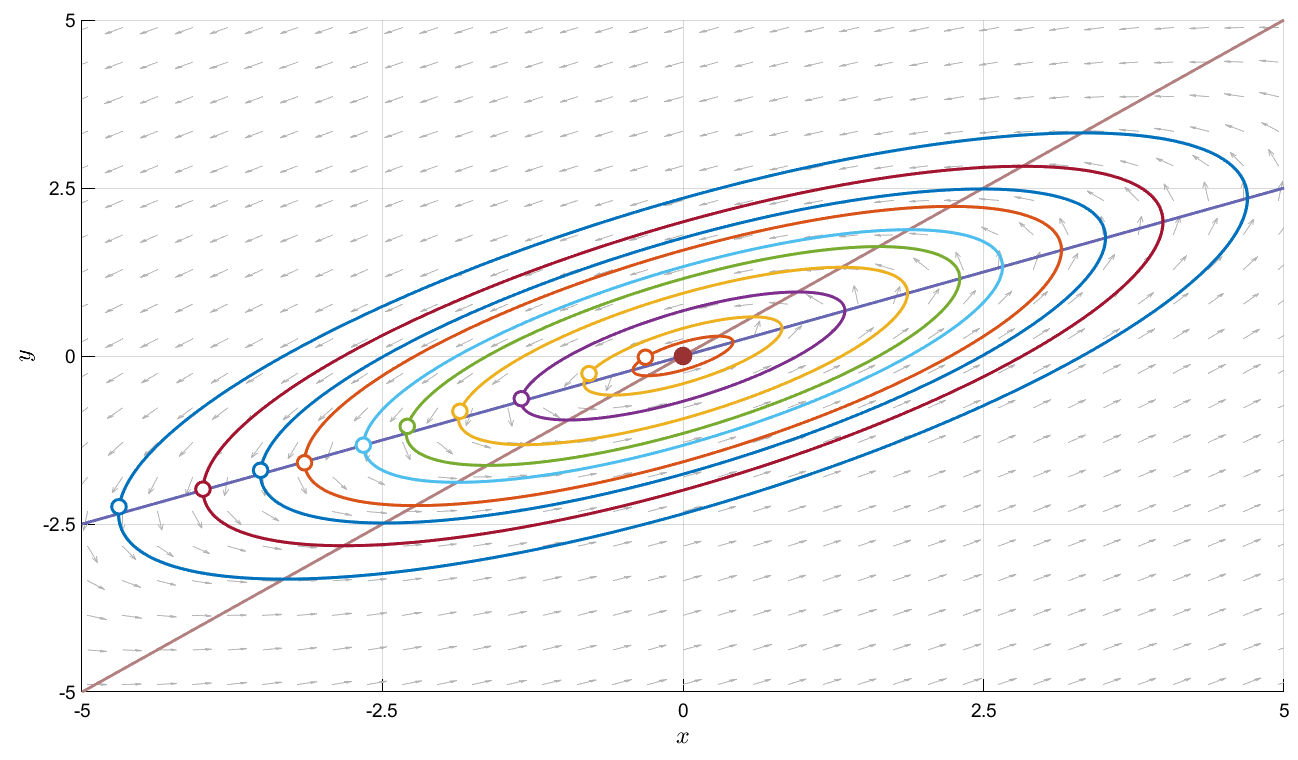
\includegraphics[width=\textwidth]{fig2.3_b.png}
        \caption{$\gamma=0$}
    \end{subfigure}
    \begin{subfigure}{.32\textwidth}
        \centering
        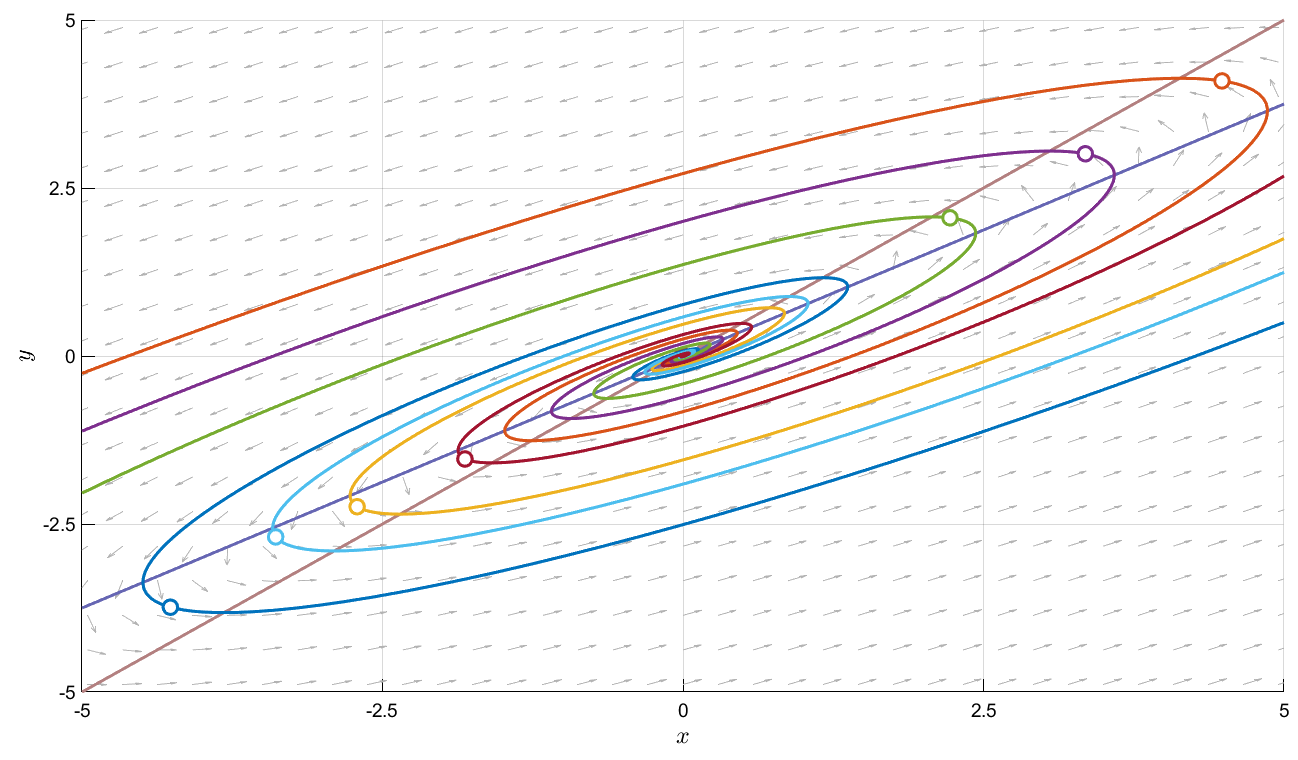
\includegraphics[width=\textwidth]{fig2.3_c.png}
        \caption{$\gamma=1/2$}
    \end{subfigure}
    \begin{subfigure}{.49\textwidth}
        \centering
        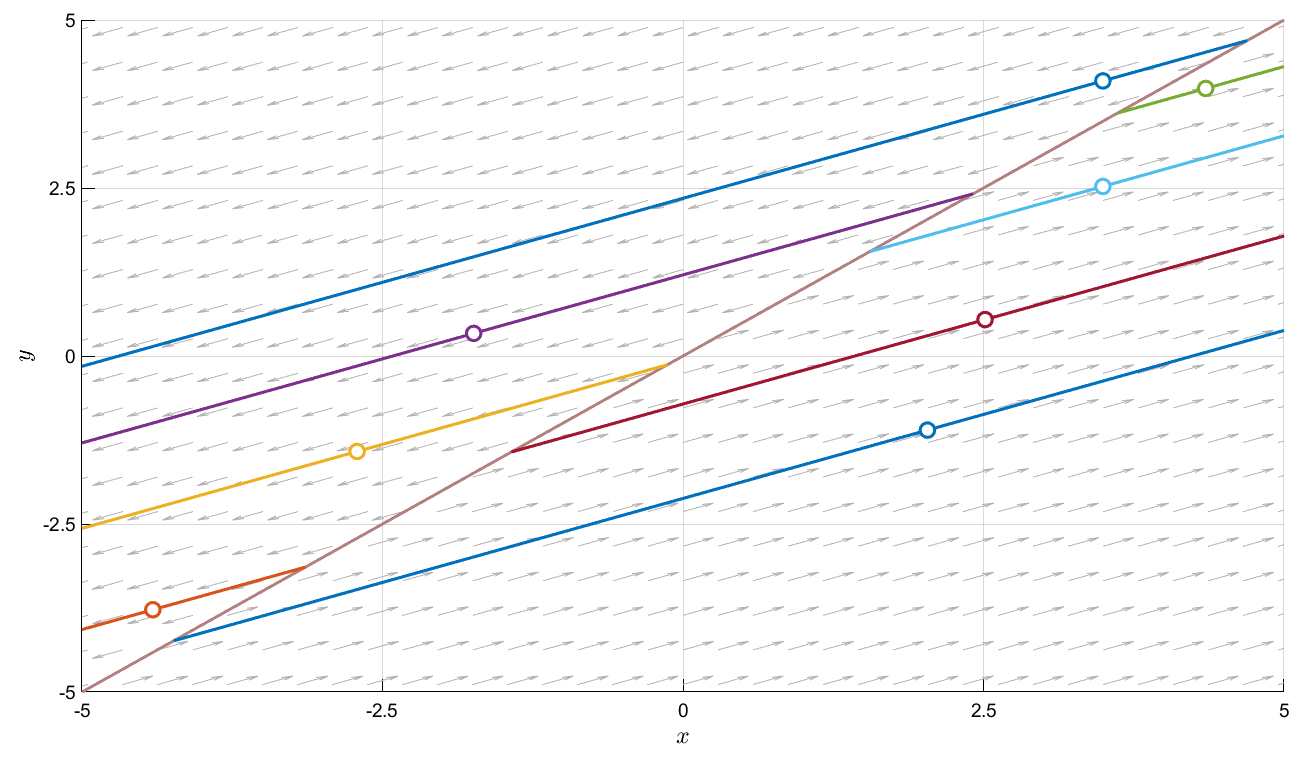
\includegraphics[width=\textwidth]{fig2.3_d.png}
        \caption{$\gamma=1$}
    \end{subfigure}
    \begin{subfigure}{.49\textwidth}
        \centering
        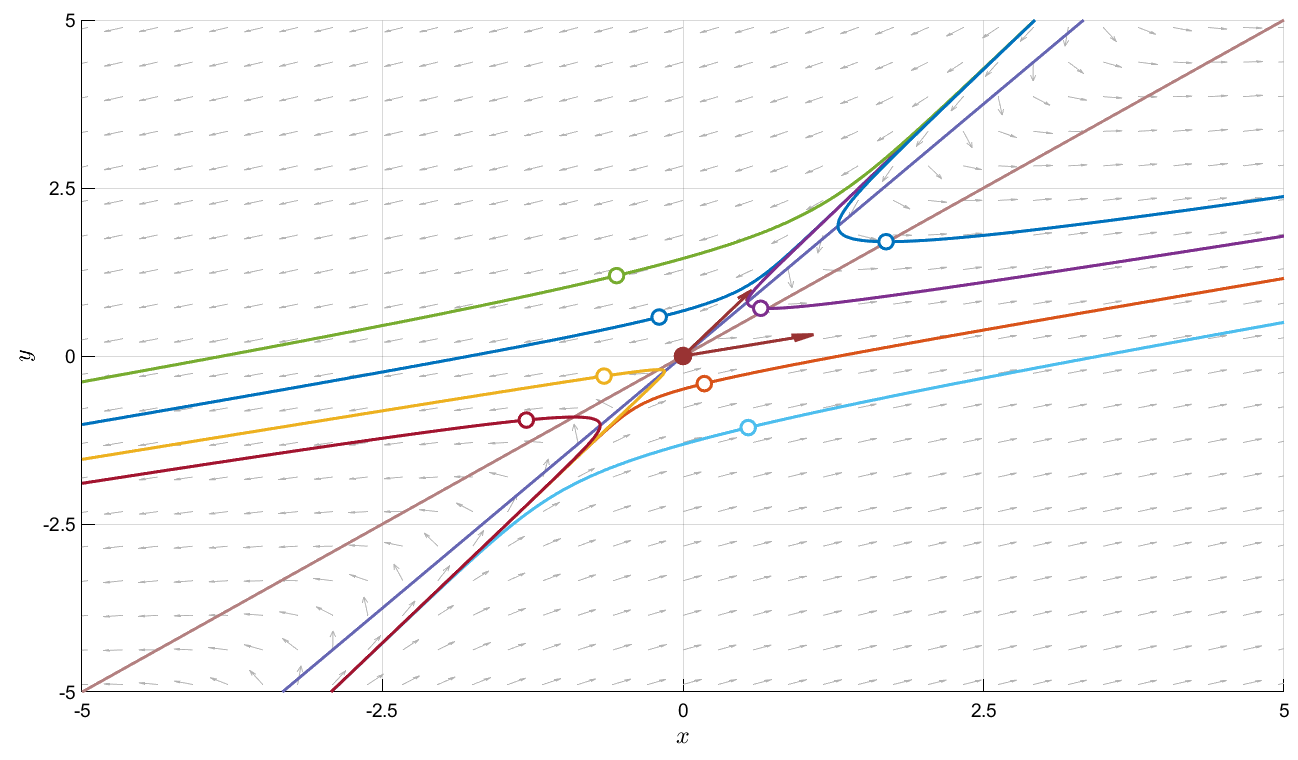
\includegraphics[width=\textwidth]{fig2.3_e.png}
        \caption{$\gamma=2$}
    \end{subfigure}
    \caption{Analysis for potential system 3}
    \label{fig:3}
\end{figure}

\begin{figure}[H]
    \centering
    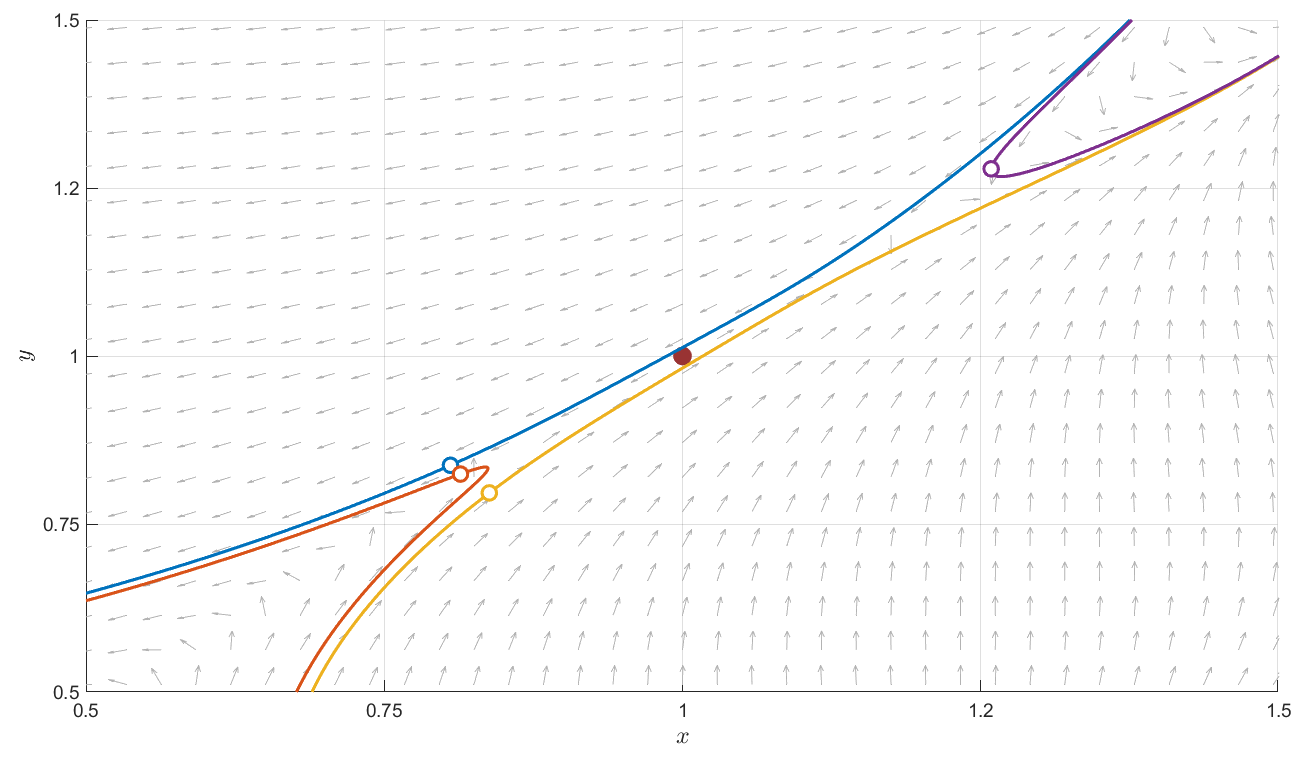
\includegraphics[width=\textwidth]{fig4.2_a.png}
    \caption{$P_3$ analysis}
    \label{fig:4}
\end{figure}

\begin{figure}[H]
    \centering
    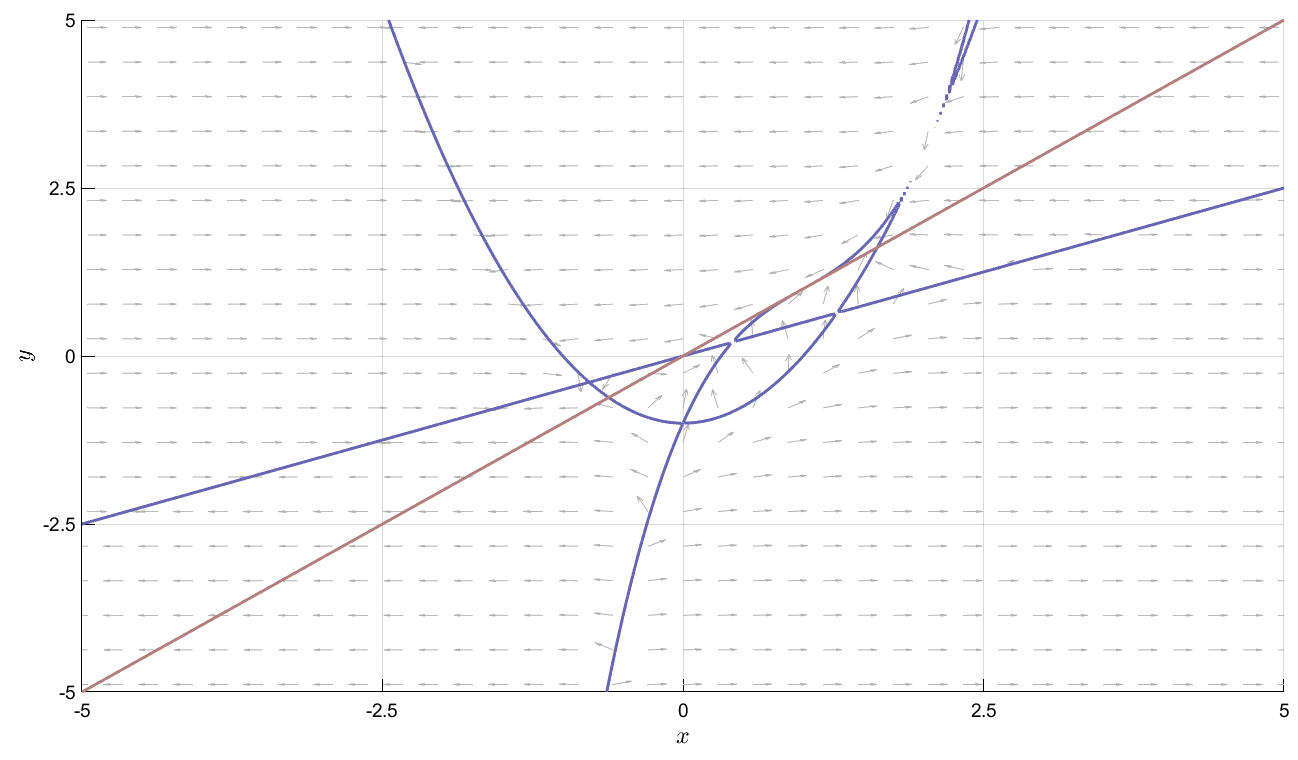
\includegraphics[width=\textwidth]{fig4.4_a.png}
    \caption{Nullclines for the system where $\alpha=-1,\beta=1,\gamma=0$}
    \label{fig:5}
\end{figure}
\begin{figure}[H]
    \centering
    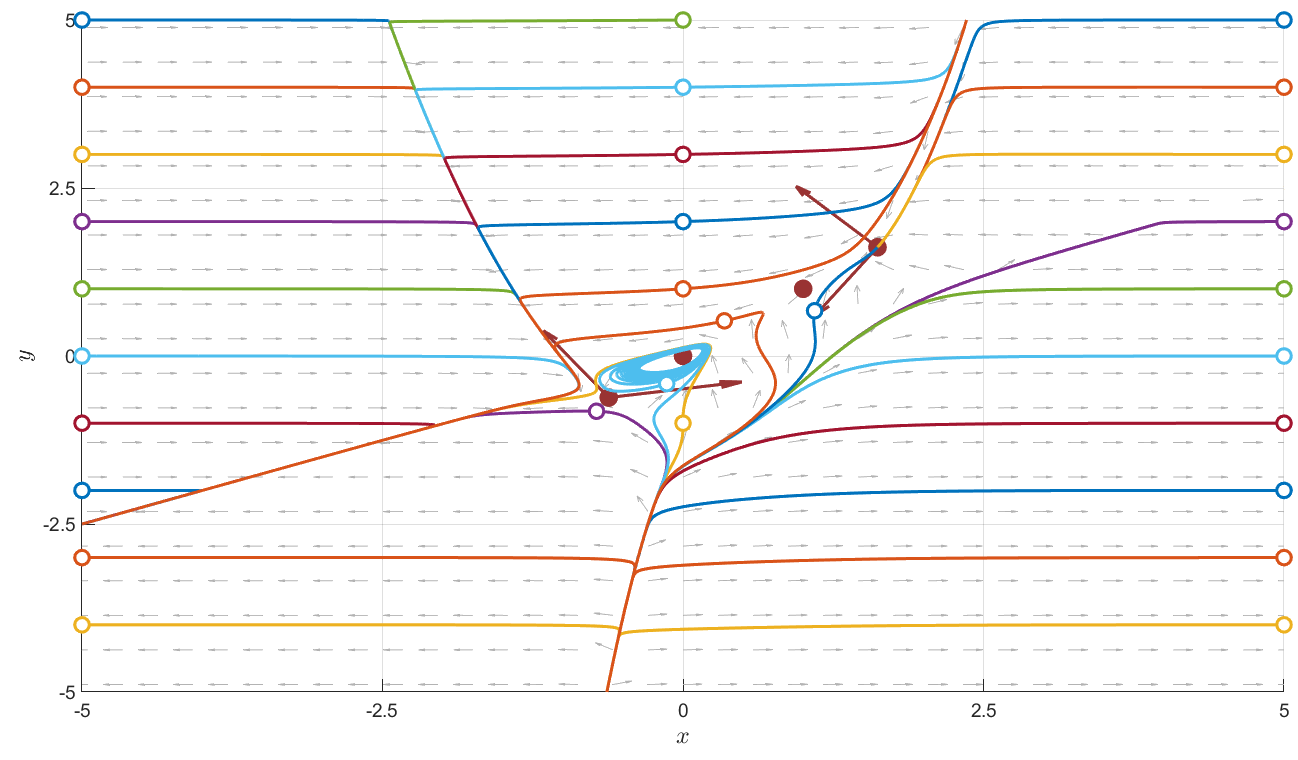
\includegraphics[width=\textwidth]{fig4.4_b.png}
    \caption{Phase portrait for the system where $\alpha=-1,\beta=1,\gamma=0$}
    \label{fig:6}
\end{figure}
\begin{figure}[H]
    \centering
    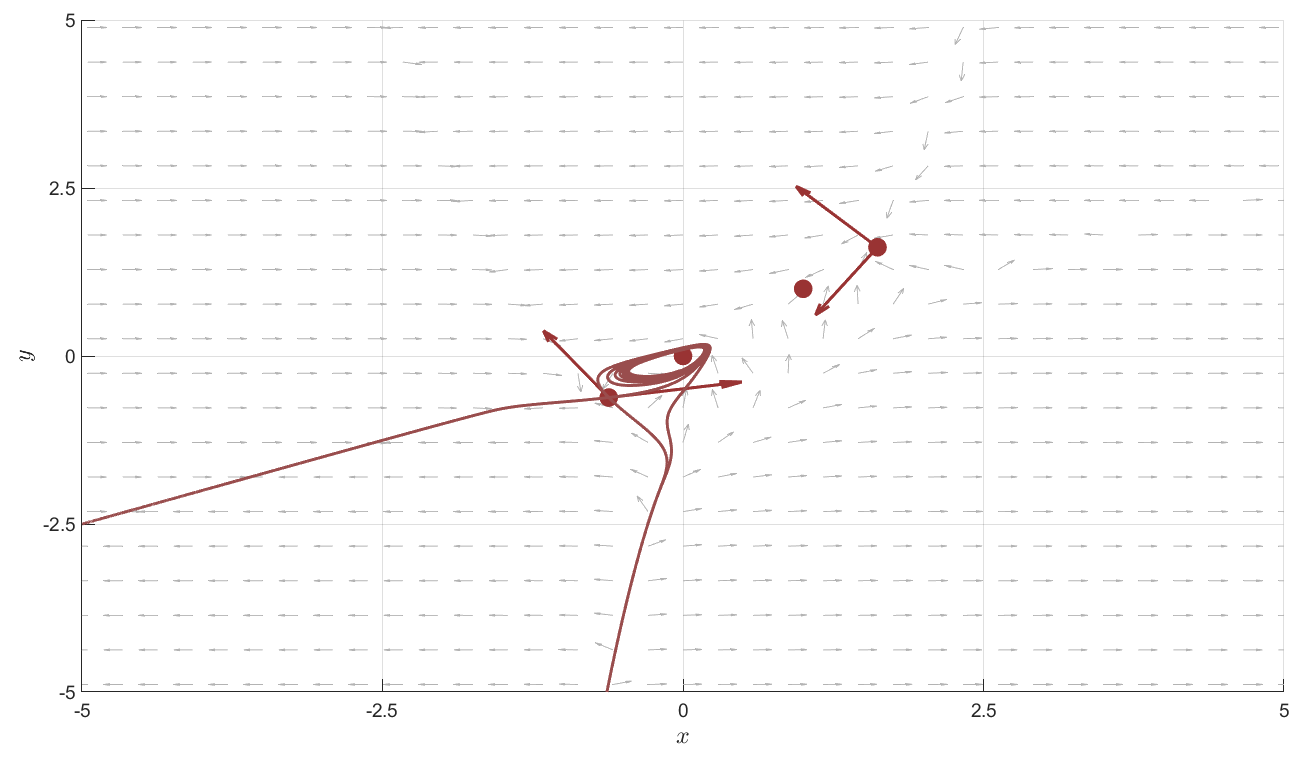
\includegraphics[width=\textwidth]{fig4.4_c.png}
    \caption{Manifolds for the system where $\alpha=-1,\beta=1,\gamma=0$}
    \label{fig:7}
\end{figure}
\begin{figure}[H]
    \centering
    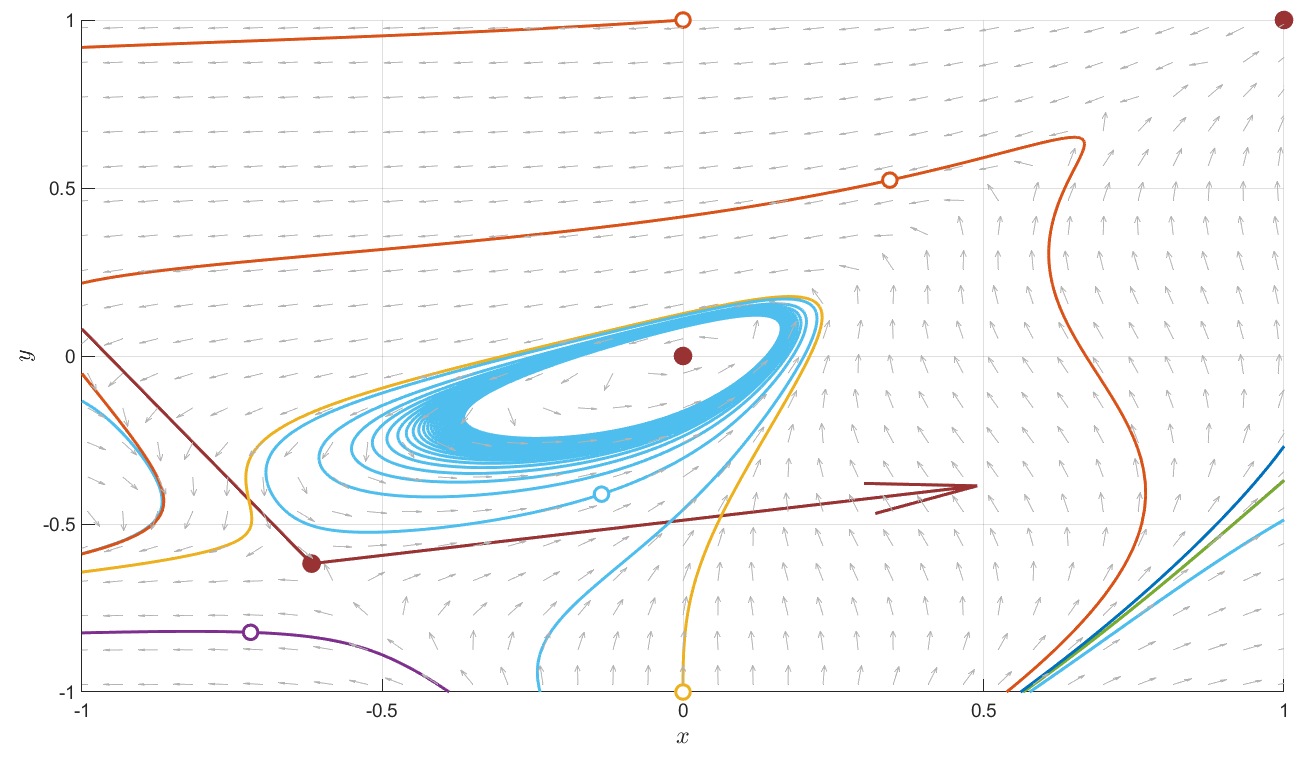
\includegraphics[width=\textwidth]{fig4.4_d.png}
    \caption{Zoomed in image of Figure~\ref{fig:6}}
    \label{fig:8}
\end{figure}

\begin{figure}[H]
    \centering
    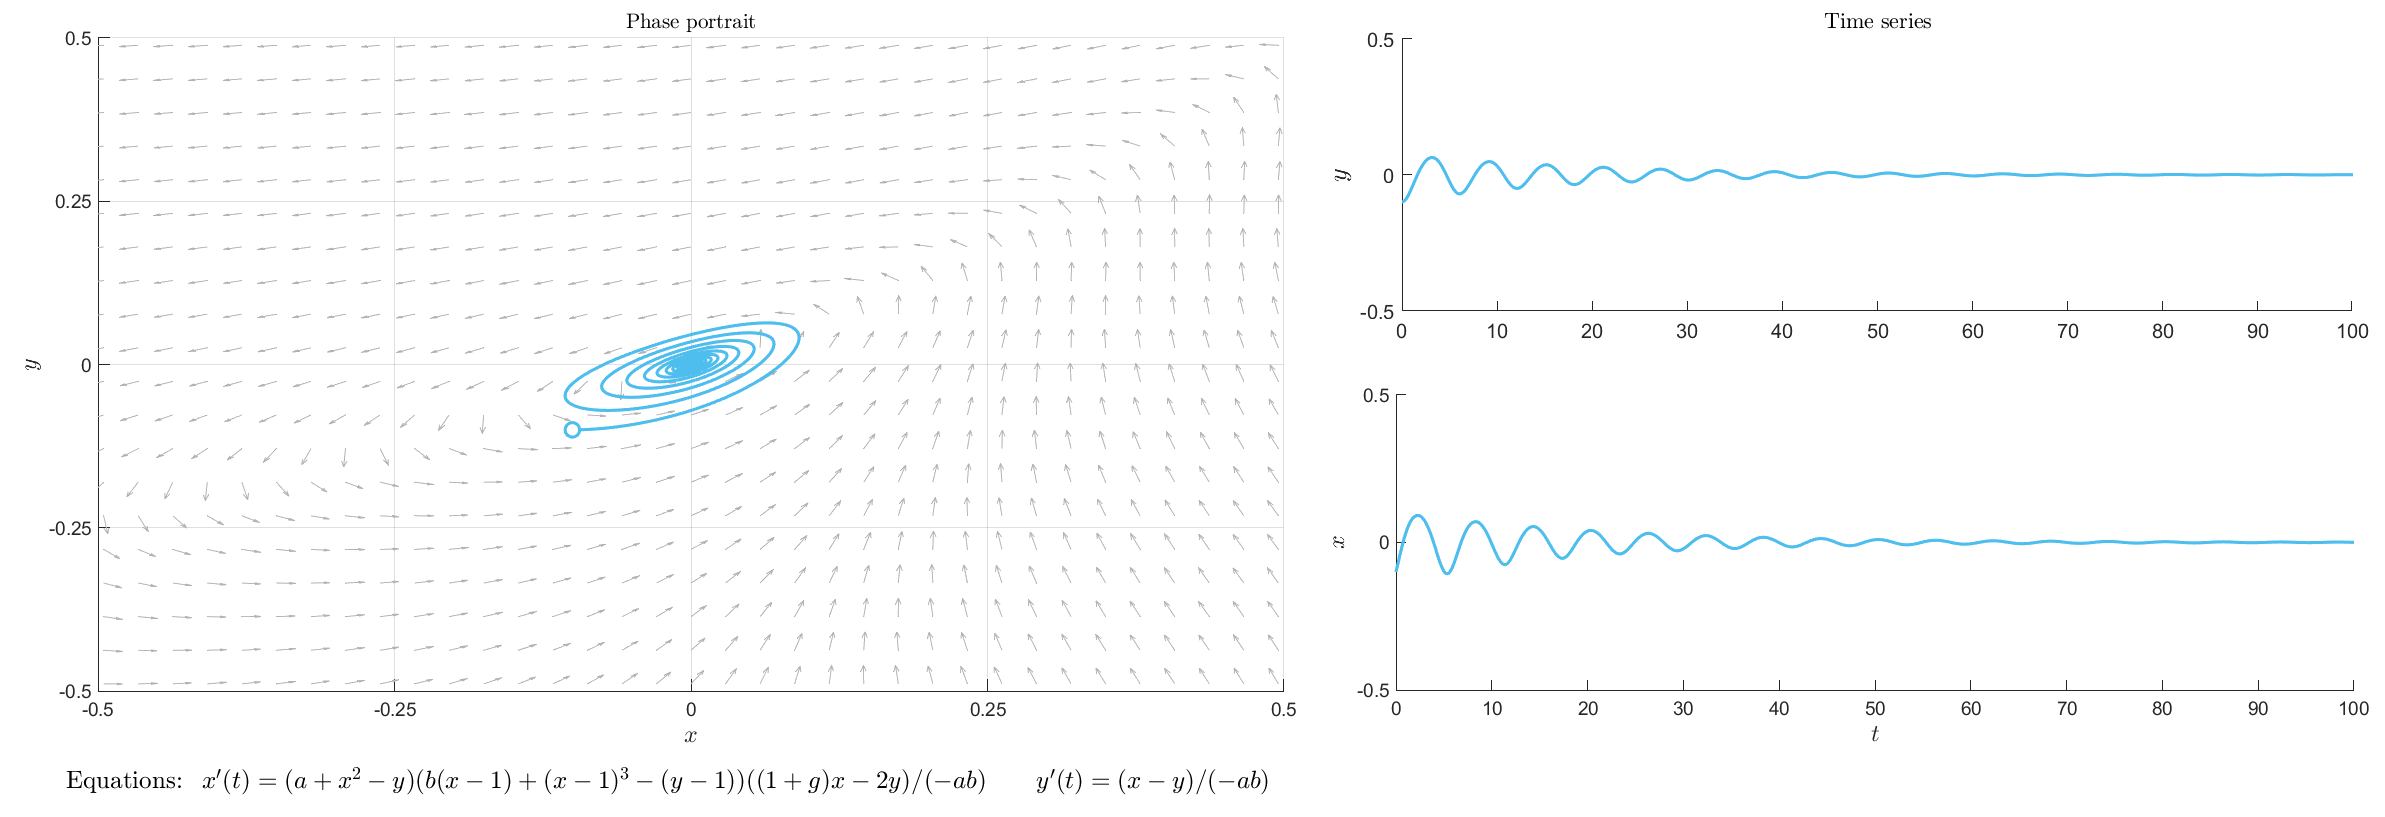
\includegraphics[width=\textwidth]{fig5.1_a.png}
    \caption{Phase portrait of the system where $\alpha=-1, \beta=1, \gamma=-0.1$}
    \label{fig:9}
\end{figure}
\begin{figure}[H]
    \centering
    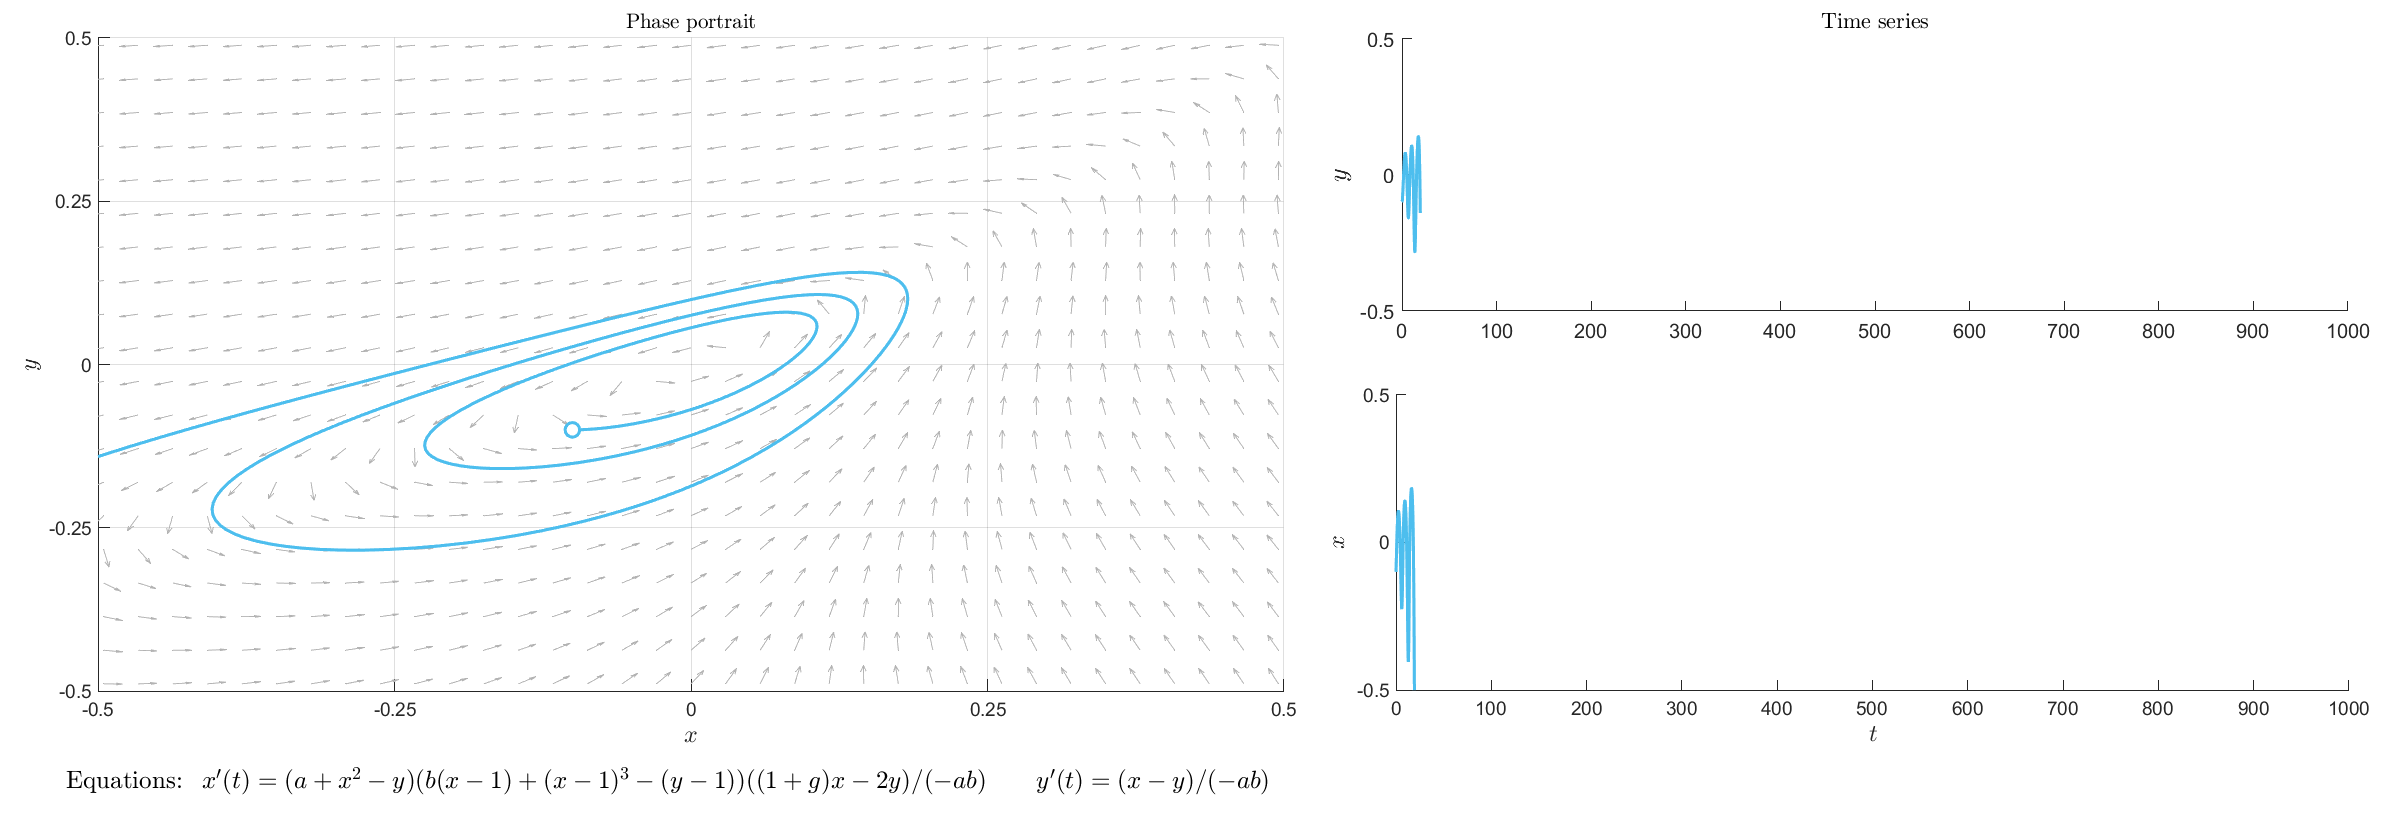
\includegraphics[width=\textwidth]{fig5.1_b.png}
    \caption{Phase portrait of the system where $\alpha=-1, \beta=1, \gamma=0.1$}
    \label{fig:10}
\end{figure}

\begin{figure}[H]
    \centering
    \begin{subfigure}{.49\textwidth}
        \centering
        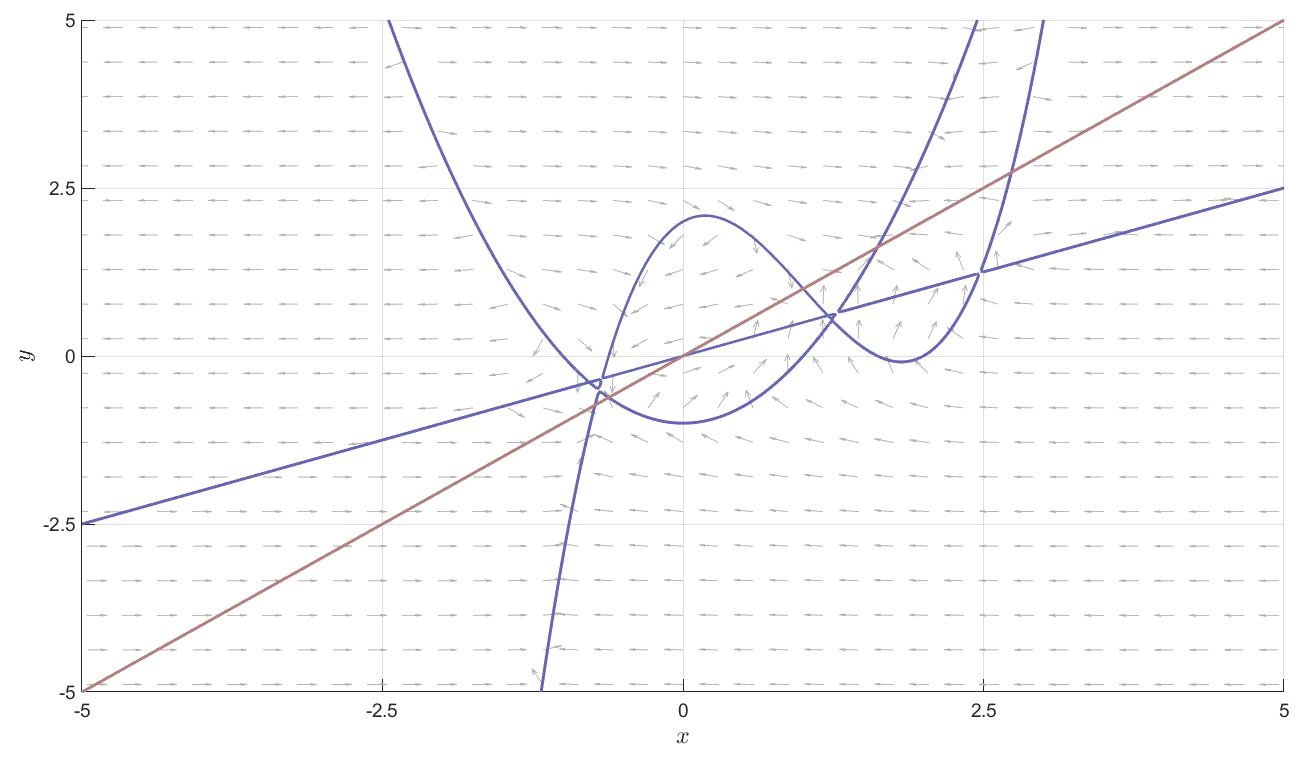
\includegraphics[width=\textwidth]{fig6.1_a.png}
        \caption{Nullclines}
    \end{subfigure}
    \begin{subfigure}{.49\textwidth}
        \centering
        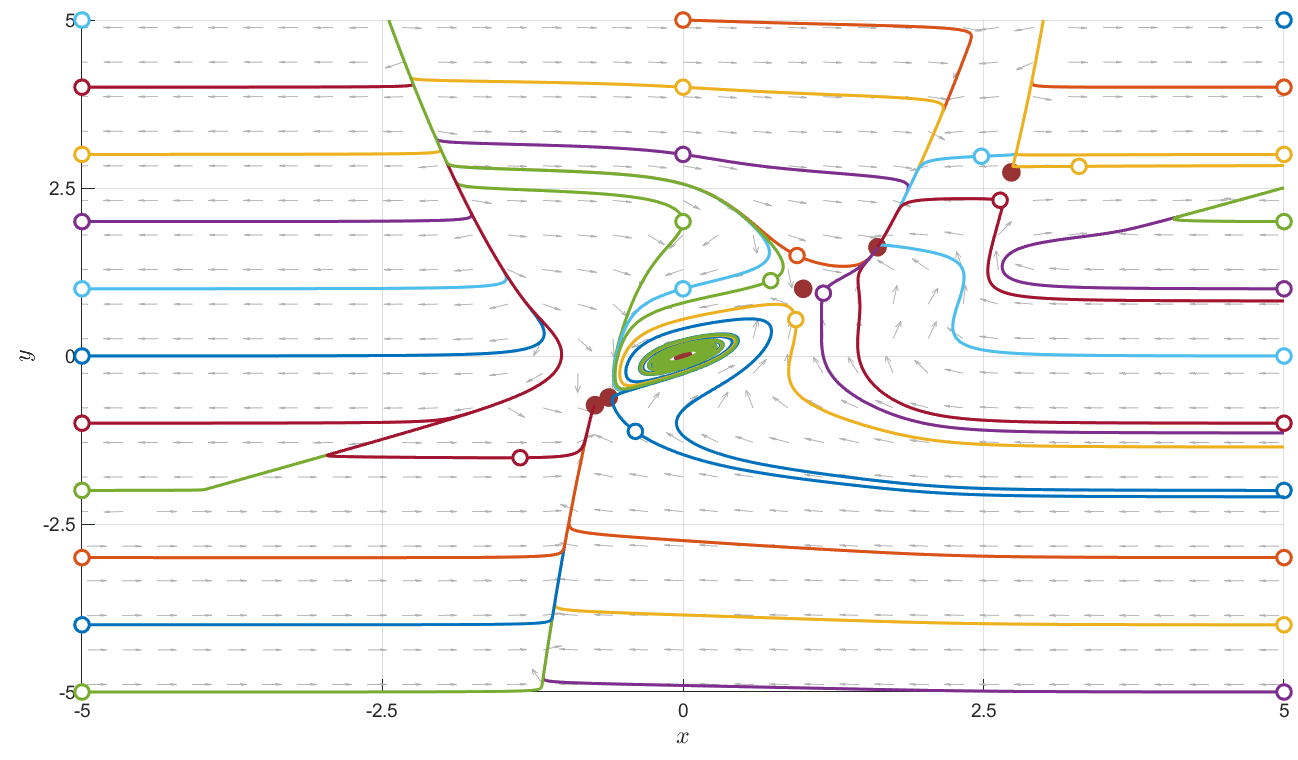
\includegraphics[width=\textwidth]{fig6.1_b.png}
        \caption{Phase Portrait}
    \end{subfigure}
    \caption{Plots for the system where $\alpha=-1, \beta=-2, \gamma=0$}
    \label{fig:11}
\end{figure}
\begin{figure}[H]
    \centering
    \begin{subfigure}{.49\textwidth}
        \centering
        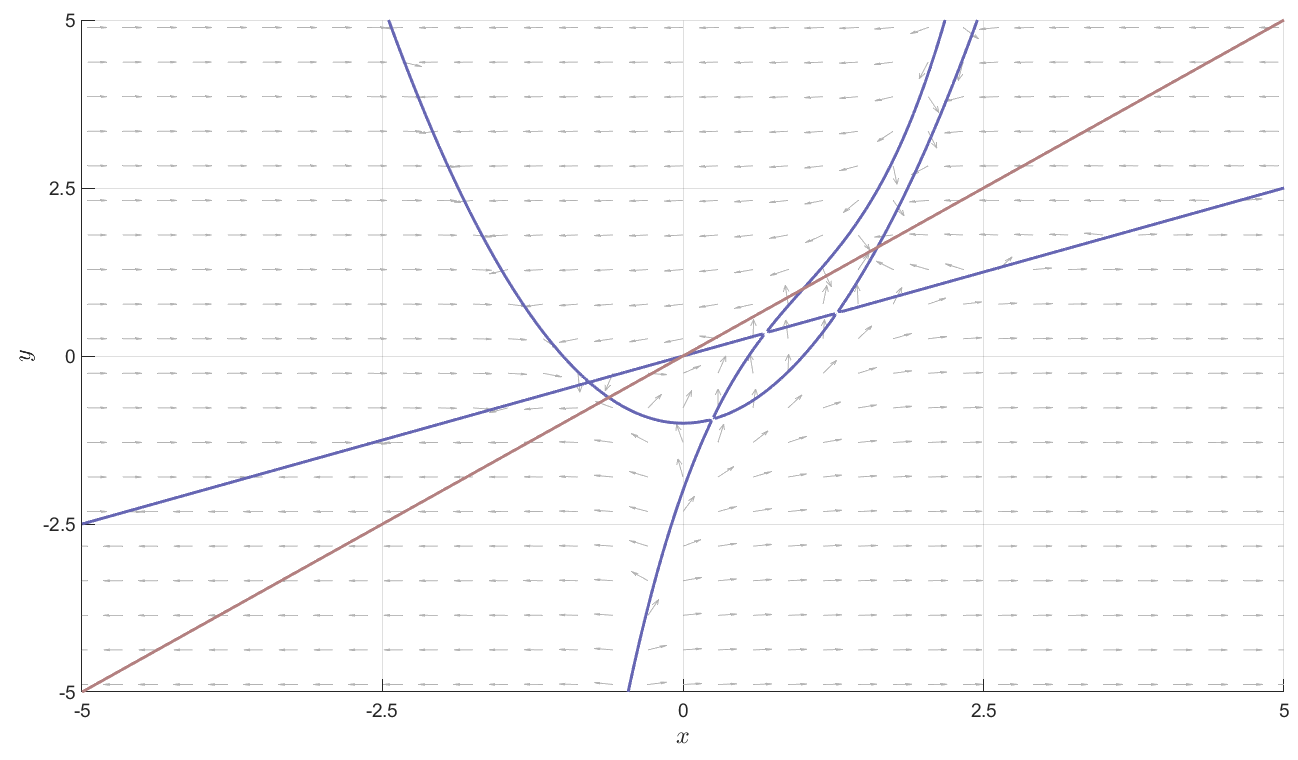
\includegraphics[width=\textwidth]{fig6.1_c.png}
        \caption{Nullclines}
    \end{subfigure}
    \begin{subfigure}{.49\textwidth}
        \centering
        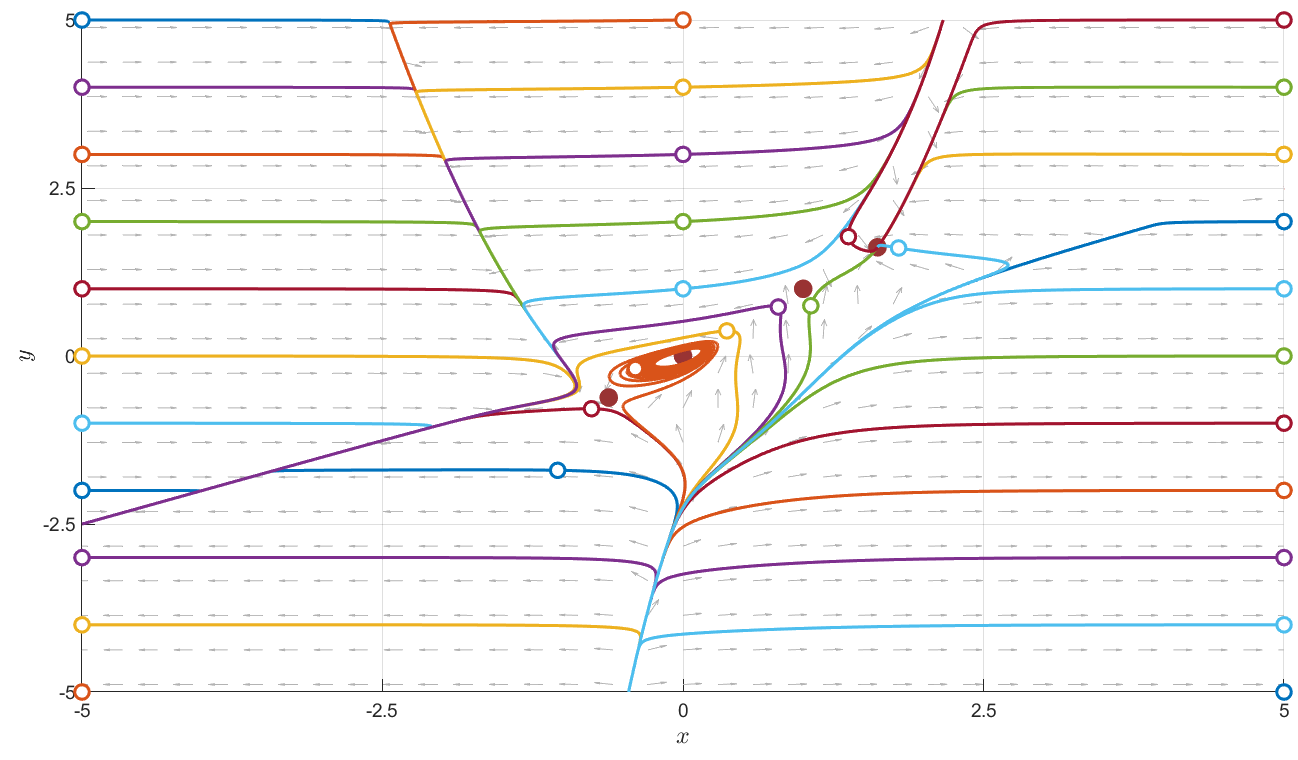
\includegraphics[width=\textwidth]{fig6.1_d.png}
        \caption{Phase Portrait}
    \end{subfigure}
    \caption{Plots for the system where $\alpha=-1, \beta=2, \gamma=0$}
    \label{fig:12}
\end{figure}


\end{document}
